
\begin{frame}{Application 2}
\end{frame}
%--------------------------------------------------------------------------------------
	\begin{frame}{Sparse Fast Fourier Transform (SFFT) Computation}
	
	 \begin{block}{Problem Statement}<1-3>
	 	\vspace{4pt}
	 	{\centering \alert{$x[n]$} : Time domain signal of length $N$ whose spectrum is $K$-sparse \\}
	\vspace{10pt} 	
	 	\centering	
	 	
	 {\large	$x[n]  \xrightarrow{\text{DFT}}  \underset{\color{blue}(K-\text{sparse})}{X[k]}$ \\}
	 	\vspace{10pt}
	 	Compute the {\alert{locations}} and \alert{values} of the $K$ non-zero coefficients w.h.p
	 \end{block}
	
	
	\only<2>{ \begin{block}{Fast Fourier Transform (FFT)}
			\begin{itemize} \itemsep1pt \parskip0pt \parsep0pt
				\item  {\color{blue} Sample complexity}:  $N$ samples
				\item  {\color{blue} Computational complexity}: $O(N \log N)$
			\end{itemize} 	          	
			\vspace{4pt}
			{\centering We want \alert{sublinear} sample and computational complexity}
			
	\end{block}}
	
	\only<3> {\begin{block}{Related work}
		\begin{itemize}
			\item Spectral estimation - Prony's method
			\item More recently Pawar and Ramchandran'13, Hassanieh, Indyk, Katabi'12
		\end{itemize}
	\end{block}}
	
	
	\end{frame}
	%--------------------------------------------------------------------------------------
	\begin{frame}{SFFT - A Sparse Graph Based Approach}
		
		\begin{block}{Main Idea - Pawar and Ramchandran 2013}
			\begin{itemize}
				\item \alert{Sub-sampling} in time corresponds to \alert{aliasing} in frequency
				\item Aliased coefficients $\Leftrightarrow$ parity check constraints of \alert{GLDPC codes}
				\item \alert{CRT} guided sub-sampling induces a code good for \alert{Peeling decoder}
                \item Problem is identical to syndrome source coding
			\end{itemize}
		\end{block}
		
		\pause
		
		\begin{block}{FFAST for Computing the DFT - Pawar and Ramchandran 2013}
			\begin{itemize}
				\item \alert{{Sampling complexity:}} $M = O(K)$ time domain samples
				\item \alert{{Computational complexity:}} $O(K \log{K})$
			\end{itemize}
		\end{block}
		
		
	%	\begin{itemize}
	%	
	%	\item Give a very simple high level description of how the problem is solved using Sparse Graph Codes (include computational complexity and number of samples in the discussion).
	%	\item Also, give an overview of how this section is going to evolve in the upcoming slides.
	%		
	%	\end{itemize}
		
	\end{frame}
	%--------------------------------------------------------------------------------------
%	\begin{frame}{SFFT - A Sparse Graph Based Approach}
%		\begin{block}{In This Talk}
%			\begin{itemize}
%				\item Aliasing and Sparse Graph Codes
%				\item \alert{F}ast \alert{F}ourier \alert{A}liasing Based \alert{S}parse \alert{T}ransform (\alert{FFAST}) algorithm
%				\item Connection between FFAST and Product Codes
%				\item Advantages of this connection
%				    \begin{itemize}
%					\item Threshold characterization
%					\item Burst analysis
%		     		\end{itemize}
%				\item Applications
%			    	\begin{itemize}
%					\item Interference-tolerant A/D Converter
%					\item GPS
%				    \end{itemize}			
%			\end{itemize}
%		\end{block}
%		
%	\end{frame}
	%-----------------------------------------------------------------------------------
	\begin{frame}{Subsampling and Aliasing - A Quick Review}
\begin{block}{Subsampling results in aliasing}
\begin{itemize}
  \item Let $x[n] \xrightarrow{N-DFT} X[k] , \ \ k,n = 0,1, \ldots,N-1$
  \item Let $x_{s}[n]  = x[mL] , \ \ m = 0,1, \ldots, N/L=M$ be a sub-sampled signal
  \item Let $x_s[m] \xrightarrow{M-DFT} X_s[l]$ be the DFT of the sub-sampled signal
  \item $\boxed{X_s[l] = M\sum\limits_{p=0}^{L-1}X[l+pM]}$
\end{itemize}
\end{block}
%		\begin{eqnarray}\nonumber
%		 &x[n] \xrightarrow{N-DFT} X[k] , \ \ &k,n = 0,1, \ldots,N-1 \\ \nonumber \vspace{15pt}
%		 &x_{s}[n]  = x[mL] , \ \ &m,l = 0,1, \ldots, M-1 \ \text{and} \ M = N/L\\ \nonumber \vspace{15pt}
%		 &x_s[m] \xrightarrow{M-DFT} X_s[l] \nonumber
%		\end{eqnarray}
%		
%        \begin{center}
%          \boxed{X_s[l] = M\sum\limits_{p=0}^{L-1}X[l+pM]}
%        \end{center}
%		\vspace{-5pt}
%		\begin{columns}
%			\hspace{5pt}
%			\column{.60\textwidth}
%			\begin{eqnarray}\nonumber
%			X_s[l]&= &\sum\limits_{m=0}^{M-1}x_s[m] e^{\frac{-j2\pi ml}{M}}
%			= \sum\limits_{m=0}^{M-1}x[mL] e^{\frac{-j2\pi ml}{M}}\\ \nonumber
%			&= &\sum\limits_{m=0}^{M-1} (\sum\limits_{k=0}^{N-1} X[k] e^{\frac{j2\pi mkL}{N}}) e^{\frac{-j2\pi ml}{M}}\\ \nonumber
%			&= &\sum\limits_{k=0}^{N-1} X[k] \sum\limits_{m=0}^{M-1}  e^{\frac{-j2\pi m(k-l)}{M}} \nonumber\\
%			&=& M\sum\limits_{p=0}^{L-1}X[l+pM] \nonumber
%			\end{eqnarray}
%			
%			\column{0.45\textwidth}{\scriptsize
%				\hspace{-1.5in}
%				  \[
%				  \sum\limits_{m=0}^{M-1} ( e^{\frac{-j2\pi l'}{M}})^{m} =
%				  \begin{cases}
%				  M,& l'=0(mod M) \\
%				  0,& l' \neq 0(mod M)
%				  \end{cases}
%				  \]}
%			
%		\end{columns}
	\end{frame}
	%--------------------------------------------------------------------------------------
	\begin{frame}{Aliasing and Sparse Graph Codes}
	%\begin{itemize}
	%
	%\item Give a simple example that explains how aliasing can induce a Sparse Graph Code.\\ \item Introduce the Tanner Graph for the induced code here (No background required since it is covered in Part I).	
	%\end{itemize}
	
		\begin{block}{}
			\begin{figure}[t]
				\centering
				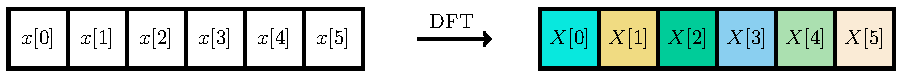
\includegraphics[width=3.1in]{./Figures/X_DFT}
			\end{figure}
		\end{block}
		
		\begin{columns}
			
			\column{.47\textwidth}
			\begin{block}{{\small $\color{red}x_s$:\ Sub-sampled by $f_1=P_1=2$}}
				\begin{figure}[t]
					\centering
					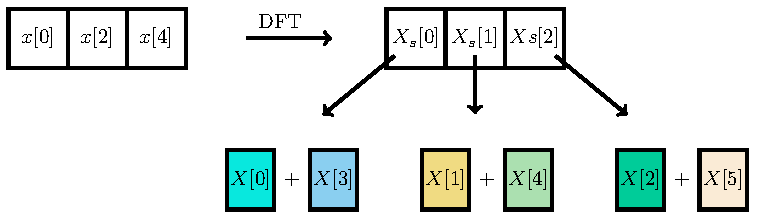
\includegraphics[width=2.3in]{./Figures/Xs}
				\end{figure}
			\end{block}
			
			\begin{block}{{\small$\color{red}z_s$:\ Sub-sampled by $f_2=P_2=3$}}
				\begin{figure}[t]
					\centering
					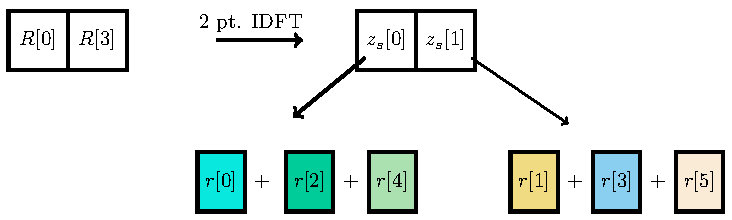
\includegraphics[width=2.3in]{./Figures/Zs}
				\end{figure}
			\end{block}
			
			\column{.47\textwidth}
			\begin{block}{\small Factor graph}
				\begin{figure}[t]
					\centering
					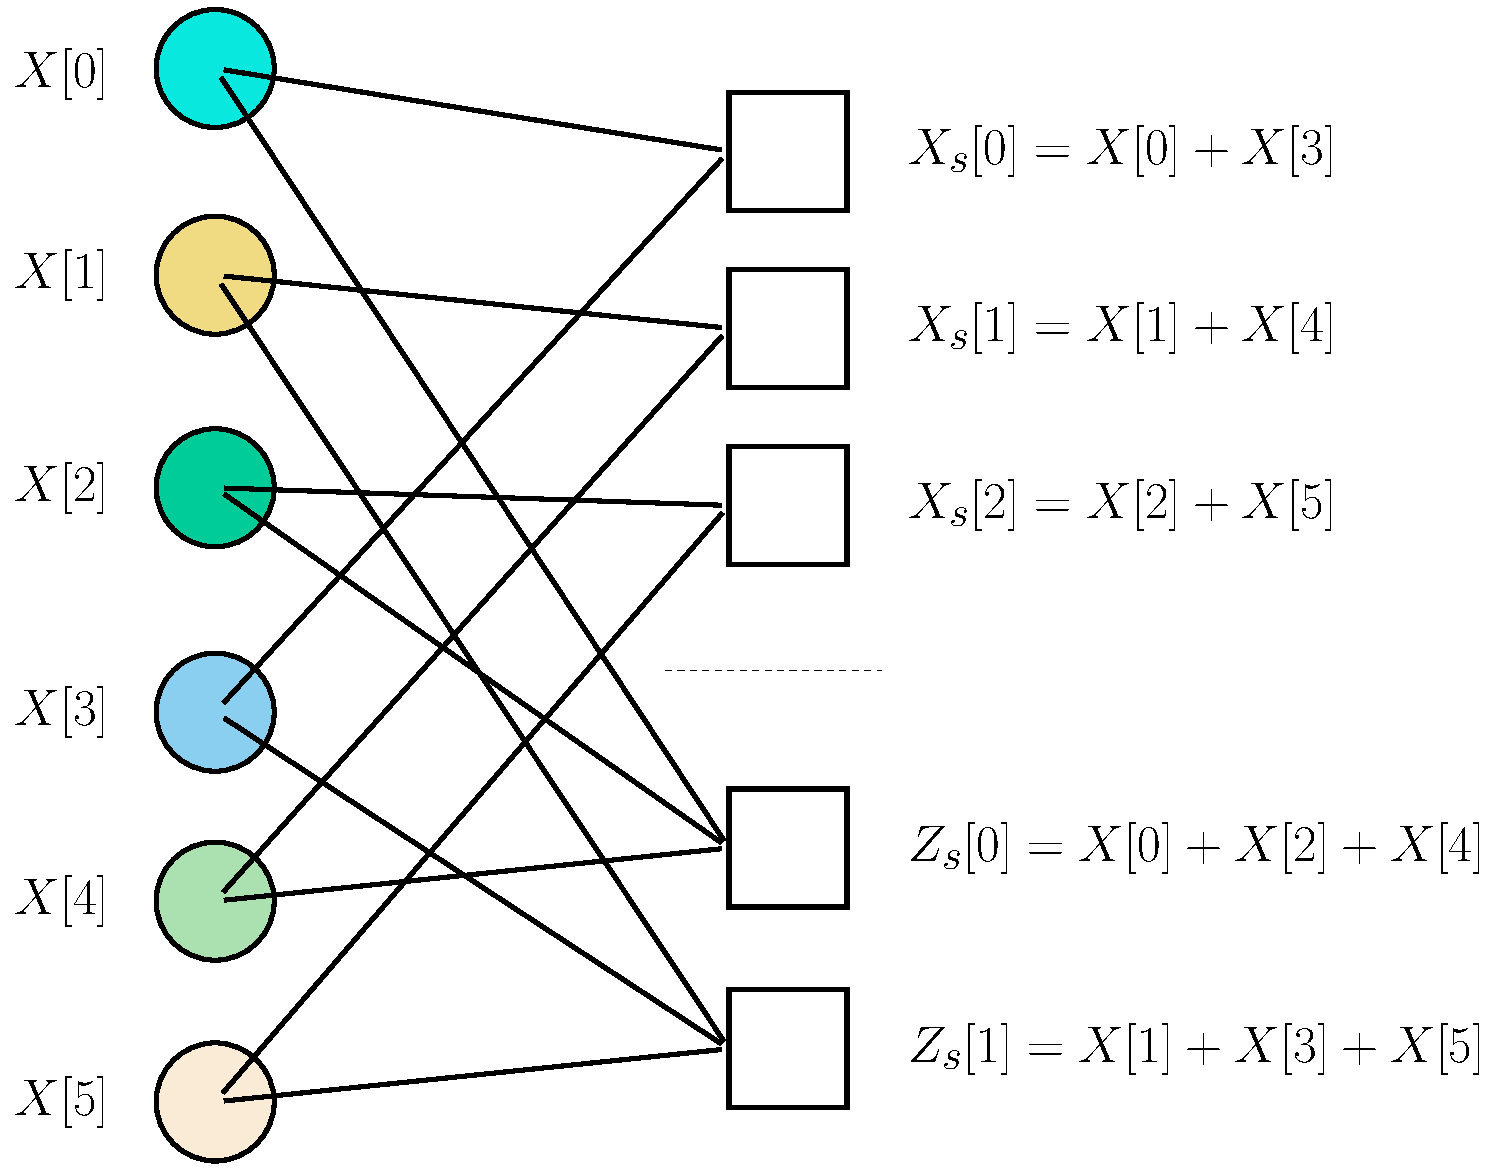
\includegraphics[width=2.3in]{./Figures/Factorgraph_example}
				\end{figure}
			\end{block}
		\end{columns}
	\end{frame}
	
	
	
	%--------------------------------------------------------------------------------------
	\begin{frame}{FFAST Algorithm Example}
	%Slide-1:
	%\begin{itemize}
	%	\item Block Diagram of a simple 2-stage FFAST setup.
	%	\item Tanner Graph of the induced code with the parity equations displayed.
	%\end{itemize}
	
	\begin{figure}[t]
		\centering
		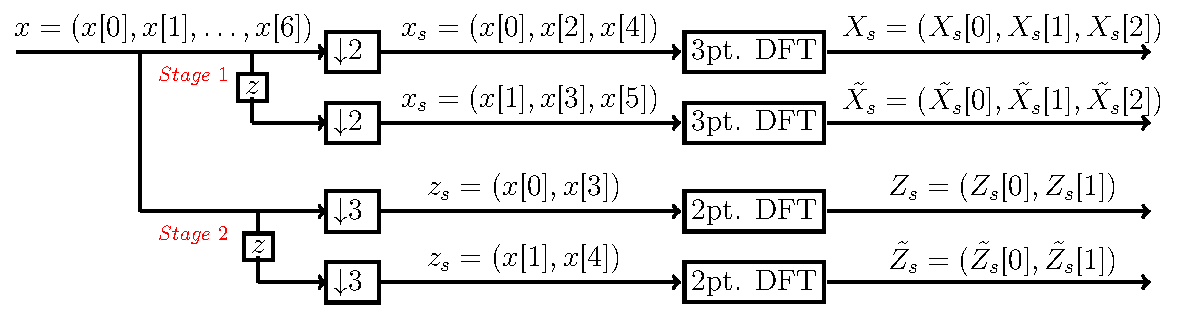
\includegraphics[width=3.6in]{./Figures/FFAST_2stages_example6}
	\end{figure}
	\vspace*{-4mm}
	\begin{figure}[t]
		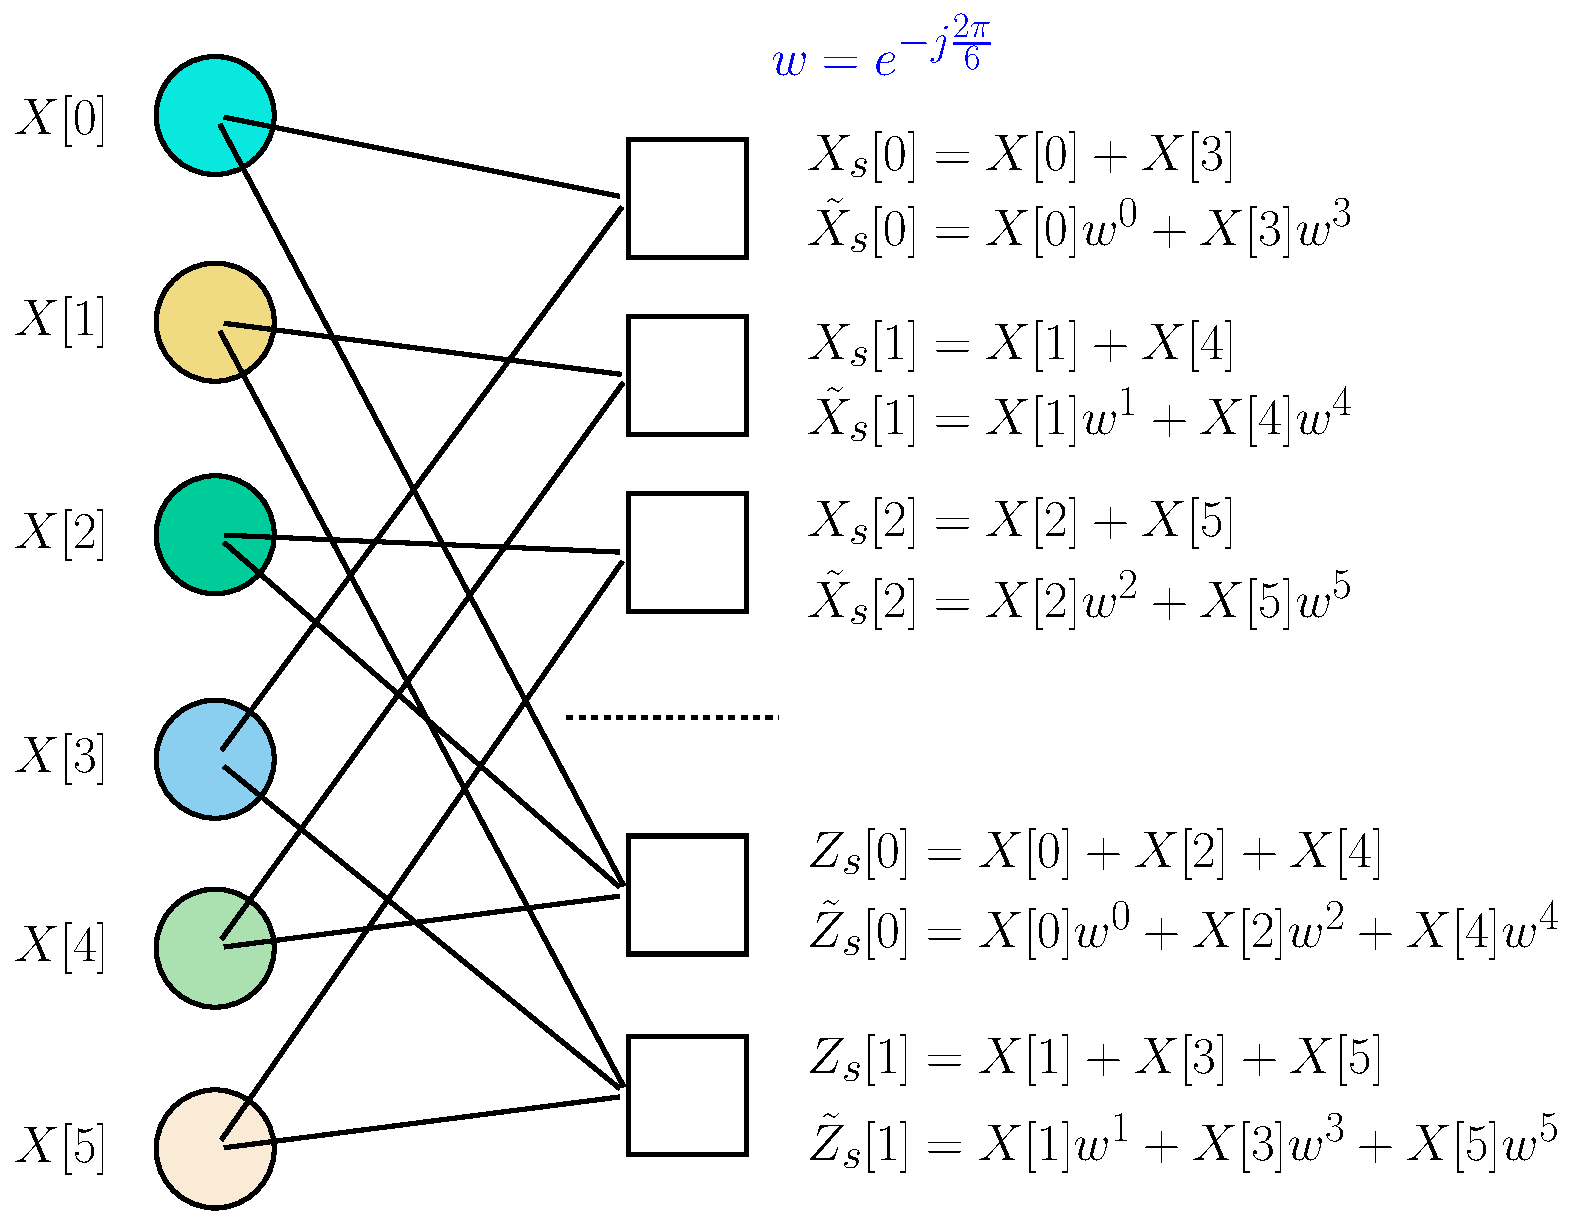
\includegraphics[width=2.9in]{./Figures/Factorgraph_example_tilde}
	\end{figure}
	
	\end{frame}
	%------------------------------------------------------------------------------------
	\begin{frame}{Singleton Detection}
			
		%Slide-2: Singleton Detection
		%\begin{itemize}
		%	\item Tanner Graph of the induced code with the equations displayed
		%	\item Simple example explaining singleton detection (ratio test)
		%	\item Summarize the singleton detection condition. {\bf(put in slide-3 if needed)}
		%\end{itemize}
		
			\vspace{-5pt}
			\begin{figure}[t]
				
				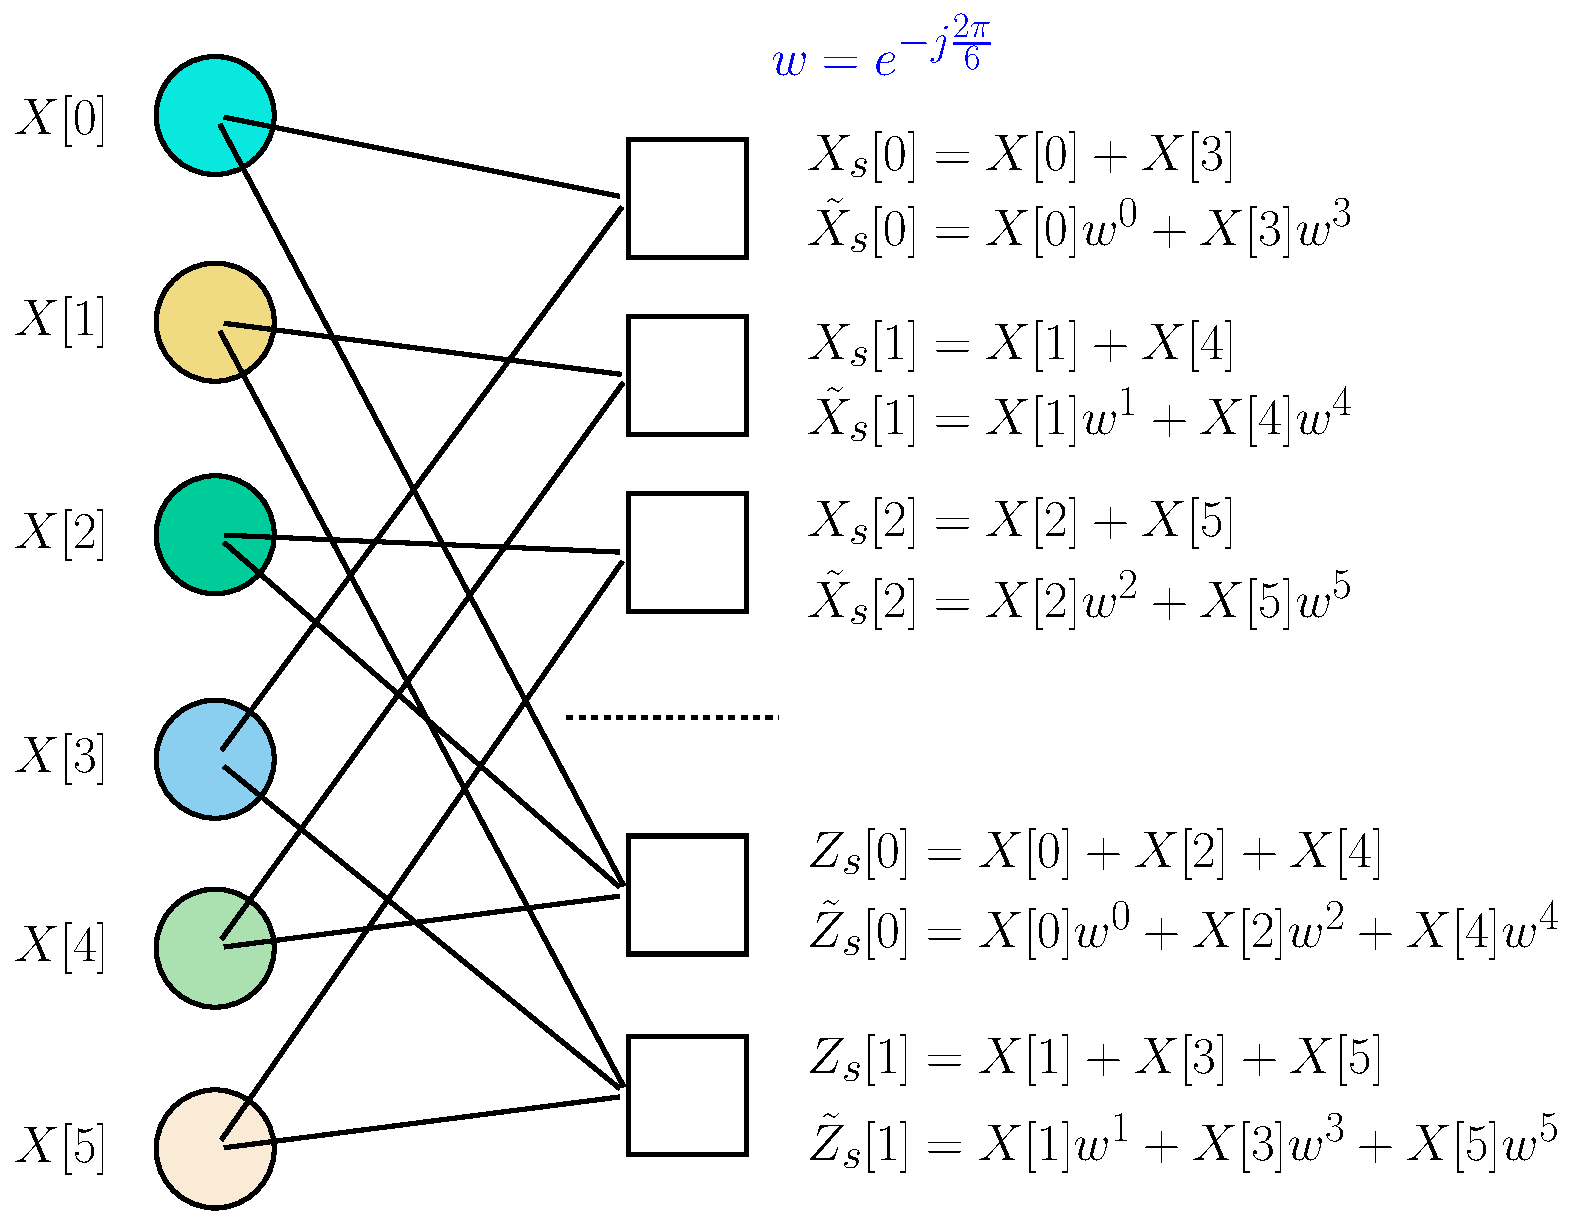
\includegraphics[width=3.0in]{./Figures/Factorgraph_example_tilde}
			\end{figure}
			\begin{block}{Singleton condition for a checknode}
			\begin{itemize}
				\item Let $i=\frac{-N}{j2\pi} \log(\frac{\tilde{X}_s[l]}{X_s[l]})$. If {\color{blue} $0 \leq i \leq N-1$}, then checknode $l$ is a \alert{Singleton}.\\
				\item $Pos(l) = i$ is the only variable node participating and $X_s[l]$ is its value.
			\end{itemize}
				
			\end{block}
			
	\end{frame}	
	%-------------------------------------------------------------------------------------
	\begin{frame}{FFAST Decoder}
		
		%Slide-3: Decoder
		%\begin{itemize}
		%	\item Tanner Graph of the induced code with the equations displayed
		%	\item Explain in few lines how the peeling decoder works for this setup
		%	\item Include a complete example with graphics that explains the complete FFAST decoder {\bf(if needed)}
		%\end{itemize}
		
%	\begin{columns}
%			\column{0.50\textwidth}
%			\begin{figure}[t]
%				\centering
%				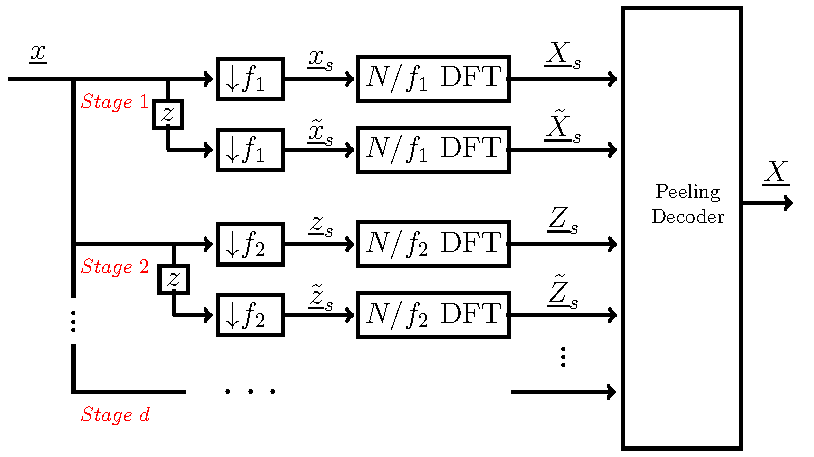
\includegraphics[width=2.5in]{./Figures/FFAST_2stages}
%			\end{figure}
%			\vspace{-6mm}
%			\hspace{-1.5in}
%			\column{0.50\textwidth}
%			
%			\begin{figure}[t]
%				
%				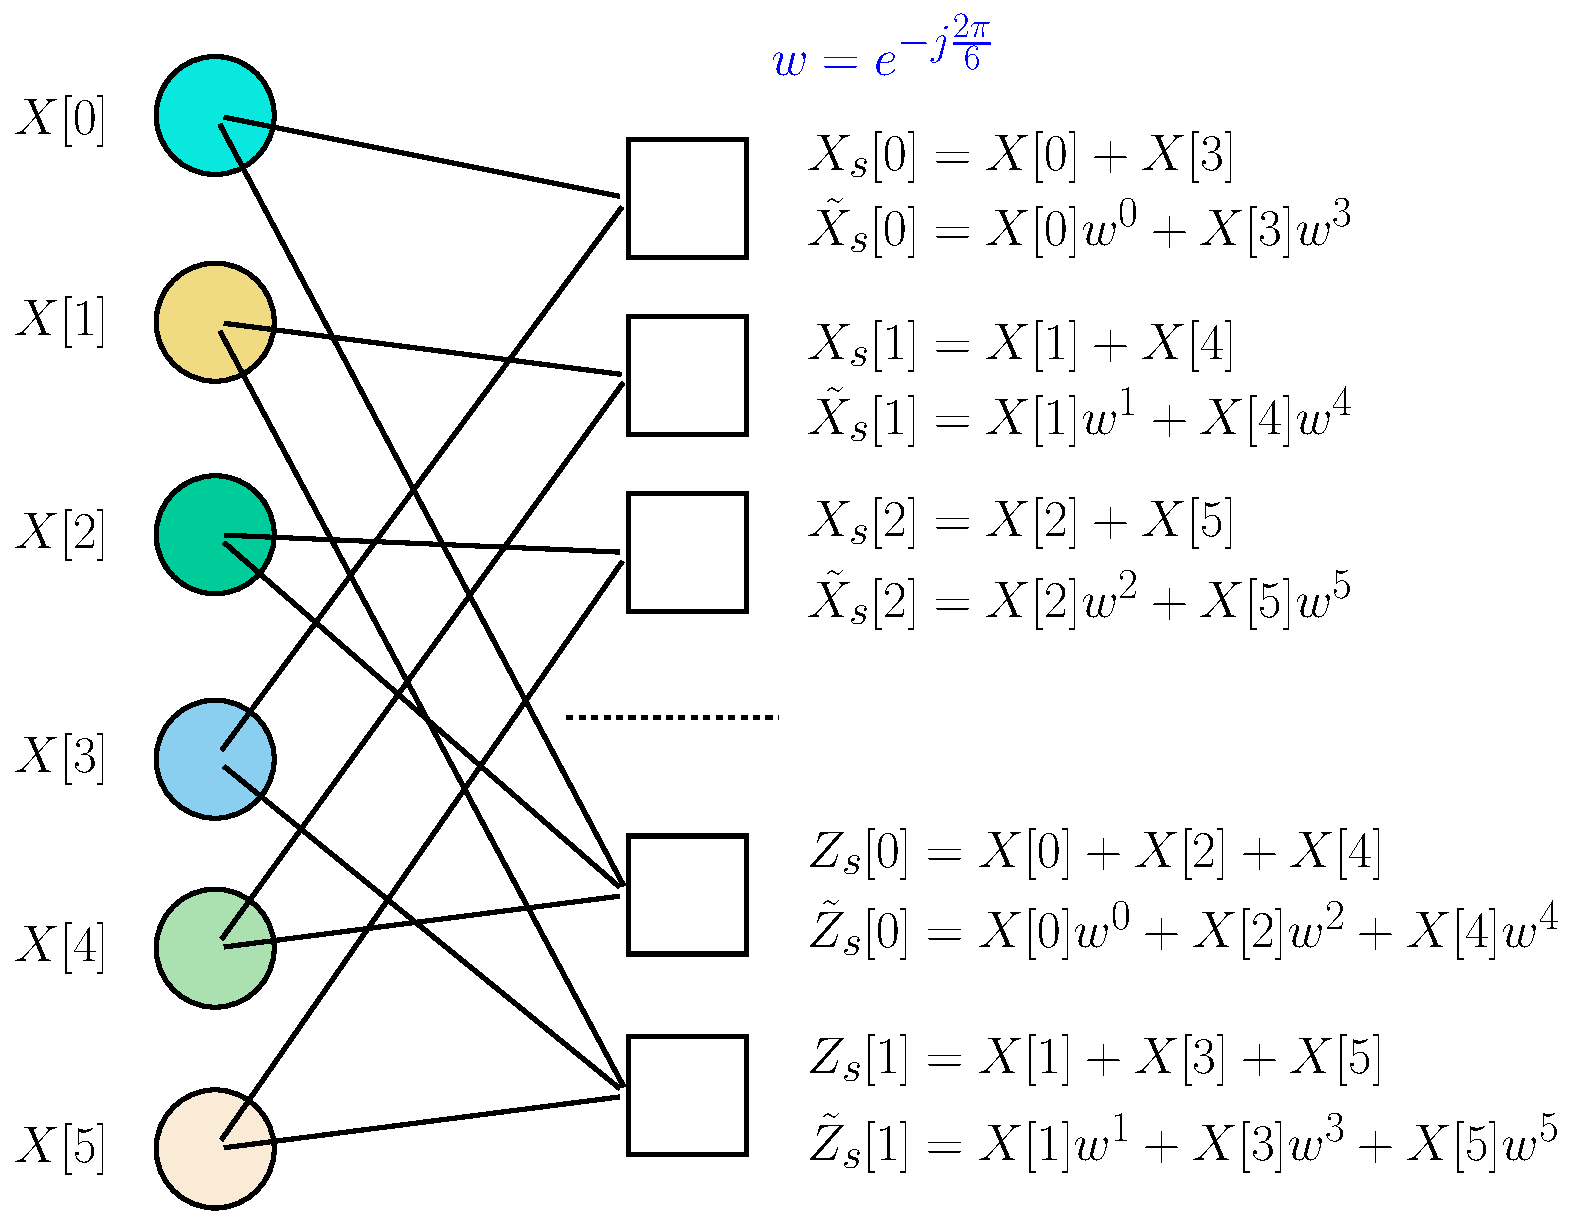
\includegraphics[width=2.45in]{./Figures/Factorgraph_example_tilde}
%			\end{figure}
%			
%		\end{columns}
			\vspace{-5pt}
			\begin{figure}[t]
				
				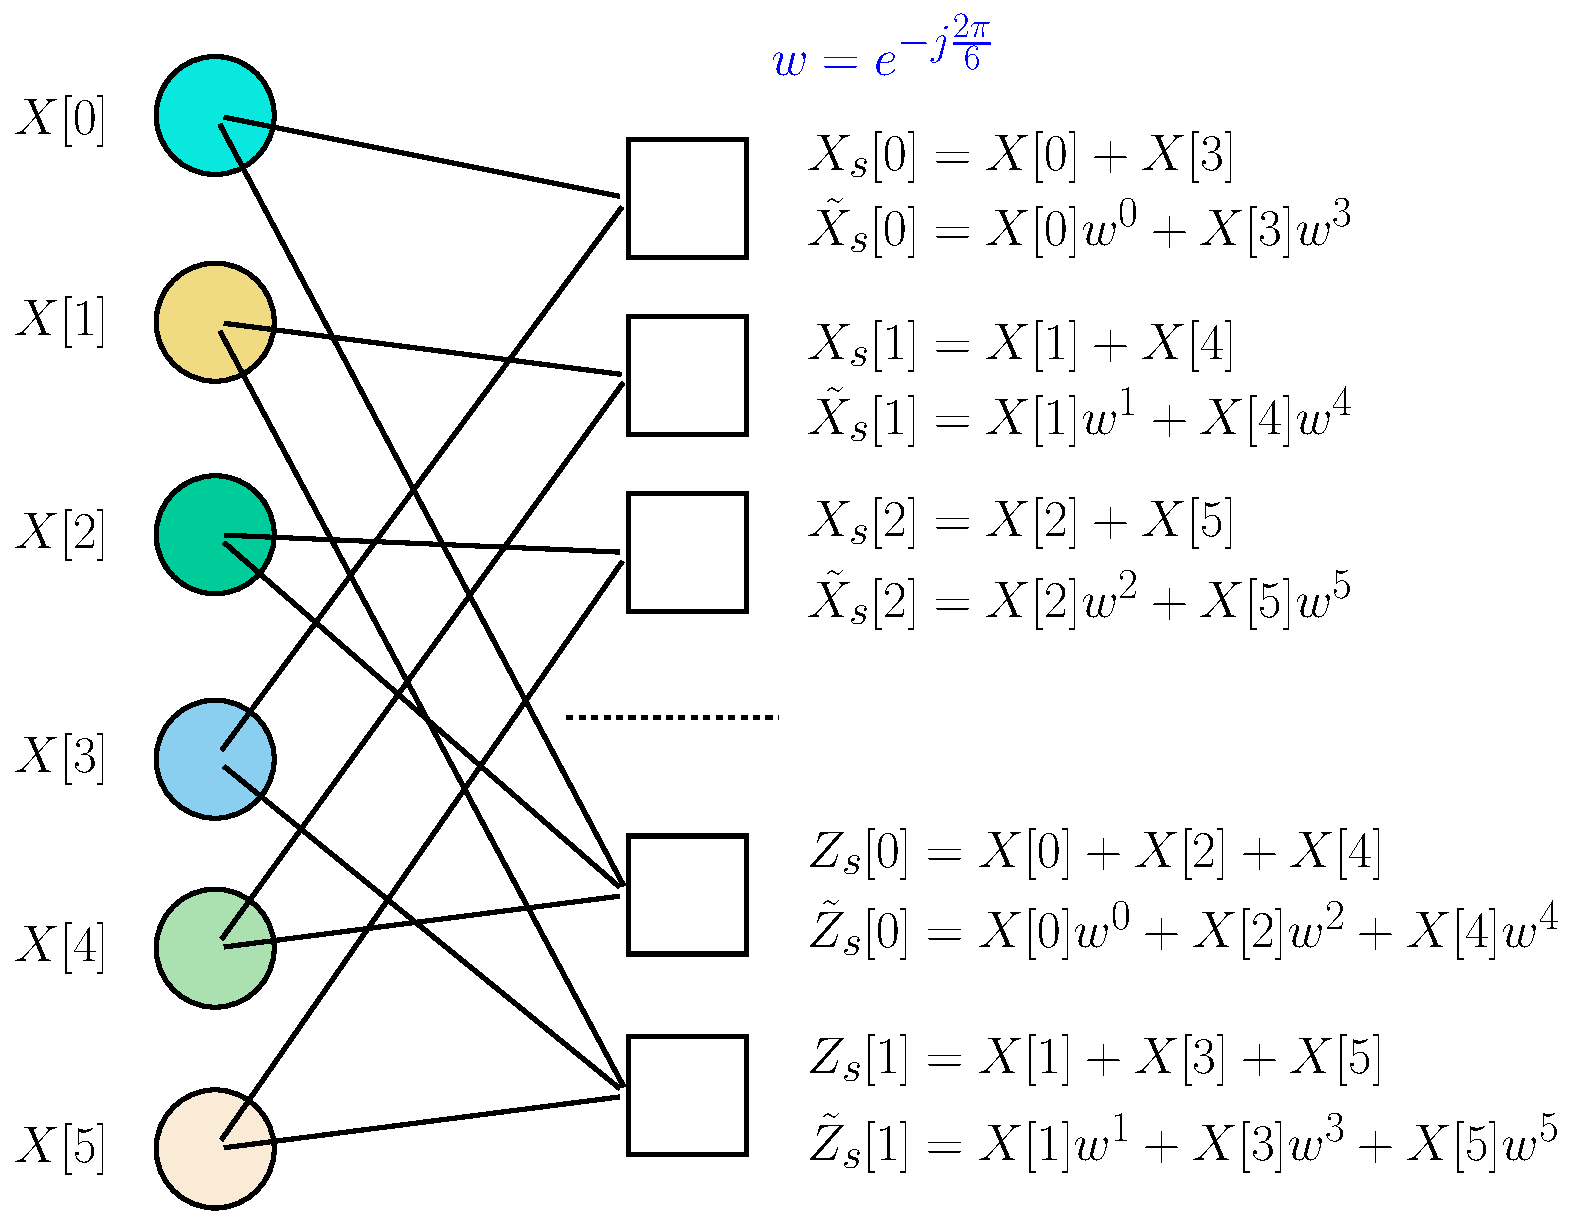
\includegraphics[width=3.0in]{./Figures/Factorgraph_example_tilde}
			\end{figure}
		\begin{block}{Peeling decoder}
			\begin{itemize}
				\item 1 non-zero value among the neighbors of any right node can be recovered
				
				\item Iteratively errors can be corrected and analyzed for random non-zero coeffs
			\end{itemize}
		\end{block}
	\end{frame}	
	%-----------------------------------------------------------------------------------------
	\begin{frame}{FFAST Decoder Example}
	\only<1-3>{\begin{block}{Example 1}
		Let $N=6$, and the non-zero coefficients be X[0]=5, X[3]=4, X[4]=7
	    \end{block}	}
	    \vspace{-7pt}
		\begin{columns}
			\only<2-3>{
				\column{0.75\textwidth}
				\begin{figure}[t]		
					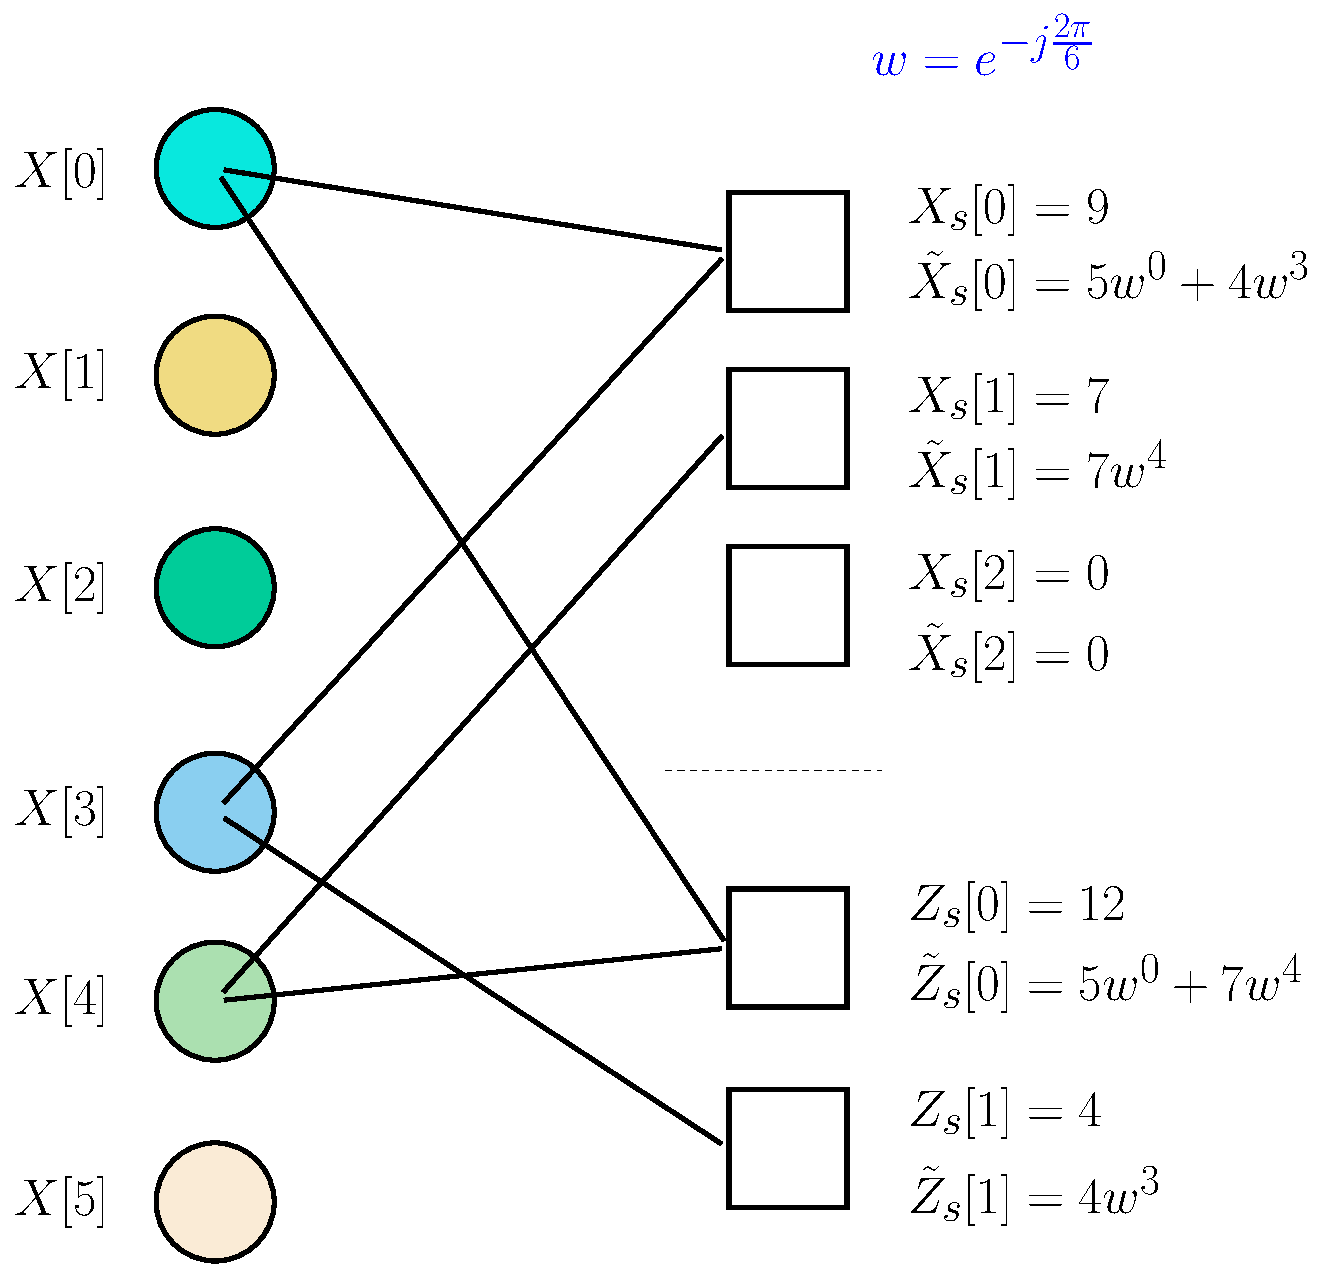
\includegraphics[width=2.6in]{./Figures/Factorgraph_example1_tilde}
				\end{figure}}
				\column{0.25\textwidth}
				\only<3>{\large \color{green} Yes, recoverable!}
				
		\end{columns}
		
		\vspace{-7pt}
		
%	\only<4-6>{
%		
%		 \begin{block}{Example 2}
%		Let $N=6$, and the non-zero coefficients be X[0] = 5,X[1] = 3 , X[2]=1, X[3] = 4, X[4] = 7.
%	     \end{block}}
%	     \begin{columns}	
%	
%	     \column{0.70\textwidth}
%	\only<5->{\begin{figure}[t]		
%			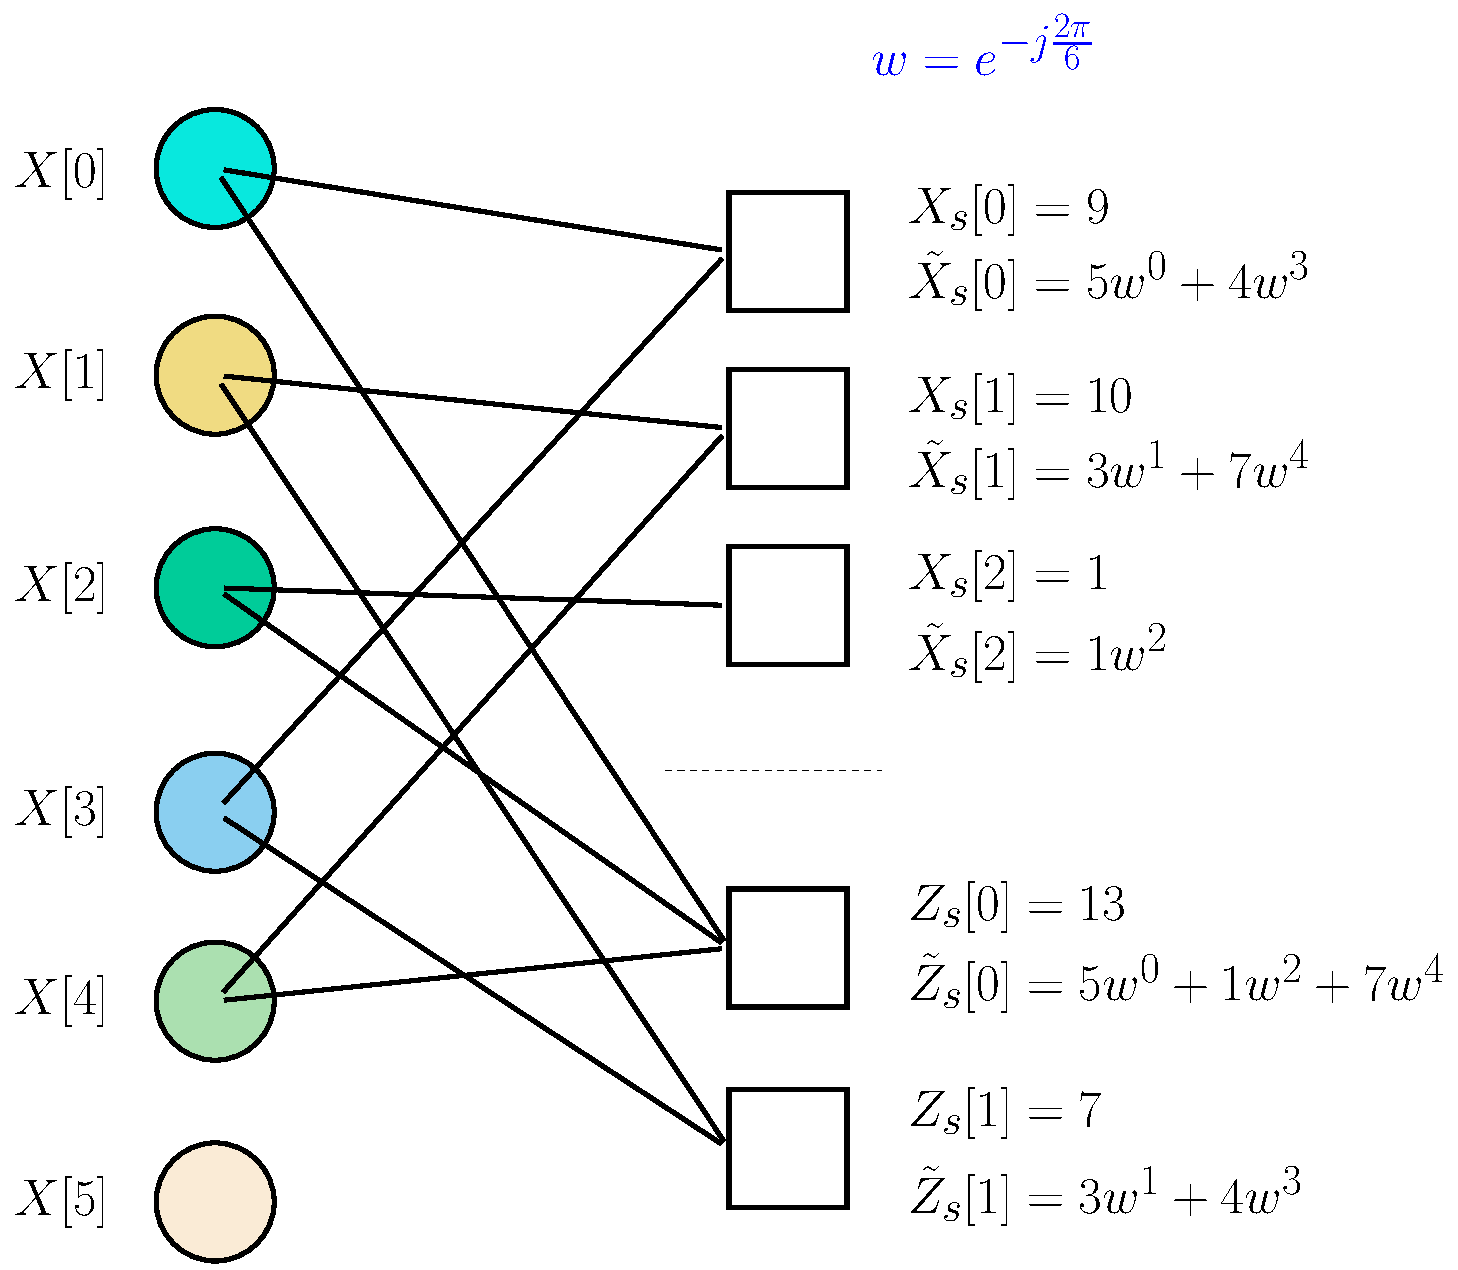
\includegraphics[width=2.6in]{./Figures/Factorgraph_example2_tilde}
%		      \end{figure}}
%	   	\column{0.30\textwidth}
%		\only<6>{\Large \alert{ Not recoverable!}}
%	\end{columns}		
	\end{frame}
%	
	%-----------------------------------------------------------------------------------------
%	\begin{frame}{FFAST Construction For Different Regimes}
%%	\begin{itemize}
%%		\item Figure: Block diagram of the a d-staged FFAST setup with generalized down-sampling parameter
%%		\item Give the values of the down-sampling parameters for less-sparse and very-sparse regime. (Also, give the aliasing equations for each case {\bf(if needed)}).
%%		\item Include the generalized FFAST construction for each $\delta$ ranges {\bf(if needed)}
%%	\end{itemize}	
%
%	\begin{figure}[t]
%		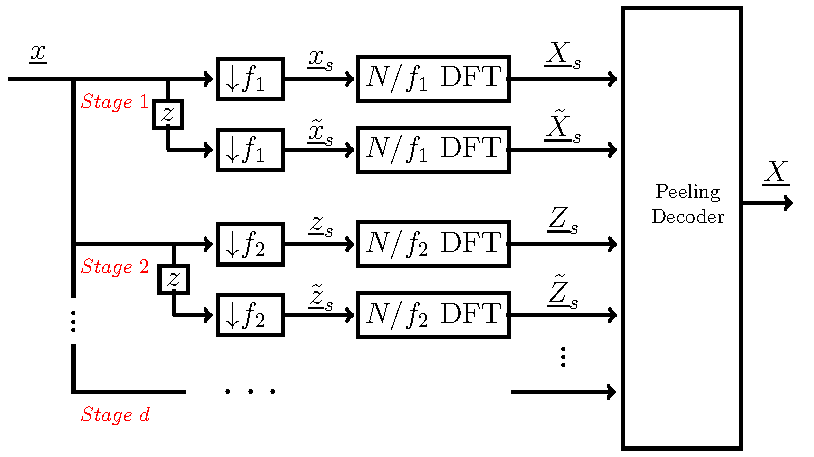
\includegraphics[width=3.0in]{./Figures/FFAST_2stages}
%	\end{figure}
%	
%	
%
%			Let, $N=P_1 \times P_2 \times \ldots P_d$
%	\begin{columns}
%		\column{0.4\textwidth}
%		
%		
%		\begin{block}{\alert{Very-sparse regime}}
%			\begin{itemize}
%				\item $K = O(N^\delta), 0<\delta \leq 1/3$
%				\item \textcolor{blue}{$f_i= N/P_i,\ i=1,2, \ldots,d$}
%				\end{itemize}
%				\end{block}
%				
%				\column{0.4\textwidth}
%				\begin{block}{\alert{Less-sparse regime}}
%					\begin{itemize}
%						\item $K = O(N^\delta), 1/3<\delta \leq 1$
%						\item \textcolor{blue}{$f_i= P_i,\ i=1,2, \ldots,d$}
%						\end{itemize}
%						\end{block}
%						
%						\end{columns}
%							
%
%			\end{frame}
	%-------------------------------------------------------------------------------------
	\begin{frame}{Generalization}
		
		%Slide-3: Decoder
		%\begin{itemize}
		%	\item Tanner Graph of the induced code with the equations displayed
		%	\item Explain in few lines how the peeling decoder works for this setup
		%	\item Include a complete example with graphics that explains the complete FFAST decoder {\bf(if needed)}
		%\end{itemize}
		
	\begin{columns}
			\column{0.50\textwidth}
			\begin{figure}[t]
				\centering
				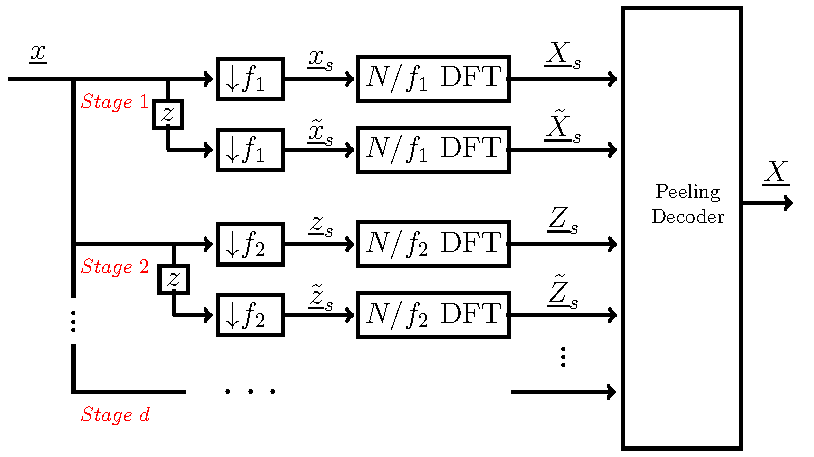
\includegraphics[width=2.5in]{./Figures/FFAST_2stages}
			\end{figure}
			\vspace{-6mm}
			\hspace{-1.5in}
			\column{0.50\textwidth}
			
			\begin{figure}[t]
				
				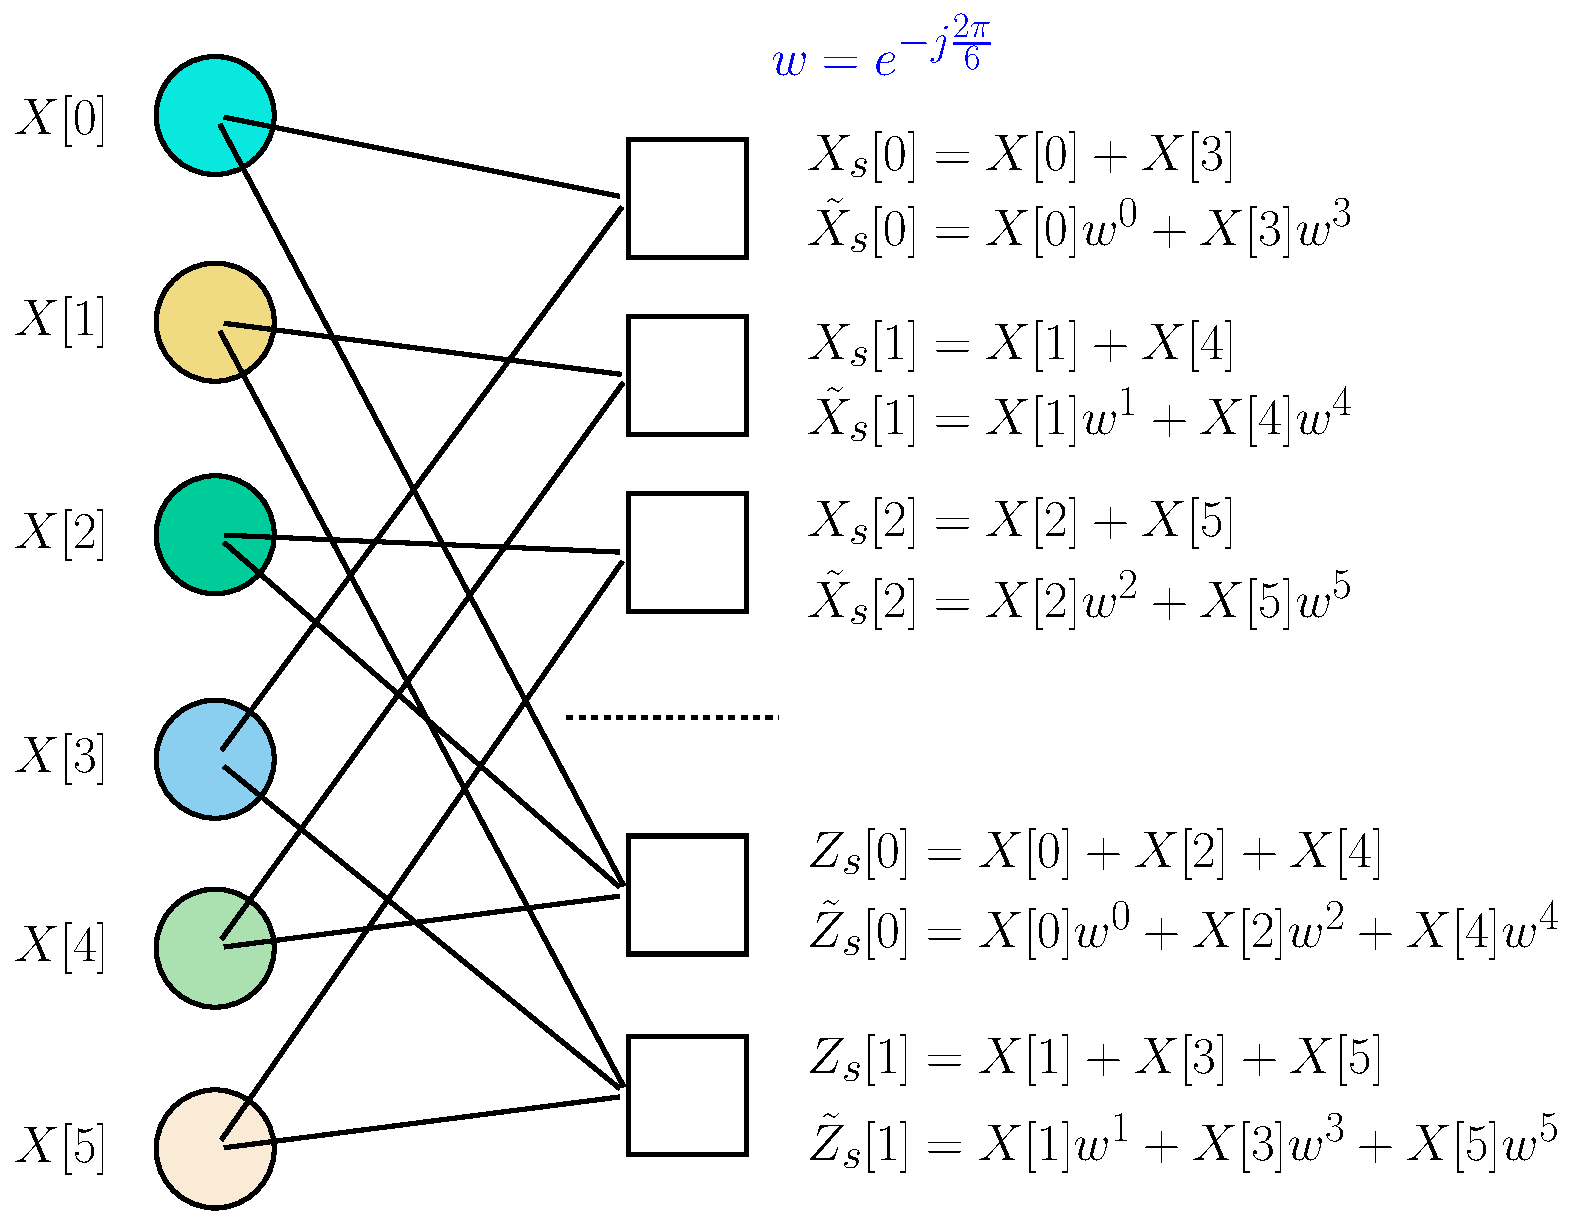
\includegraphics[width=2.45in]{./Figures/Factorgraph_example_tilde}
			\end{figure}
			
		\end{columns}
%			\vspace{-5pt}
%			\begin{figure}[t]
%				
%				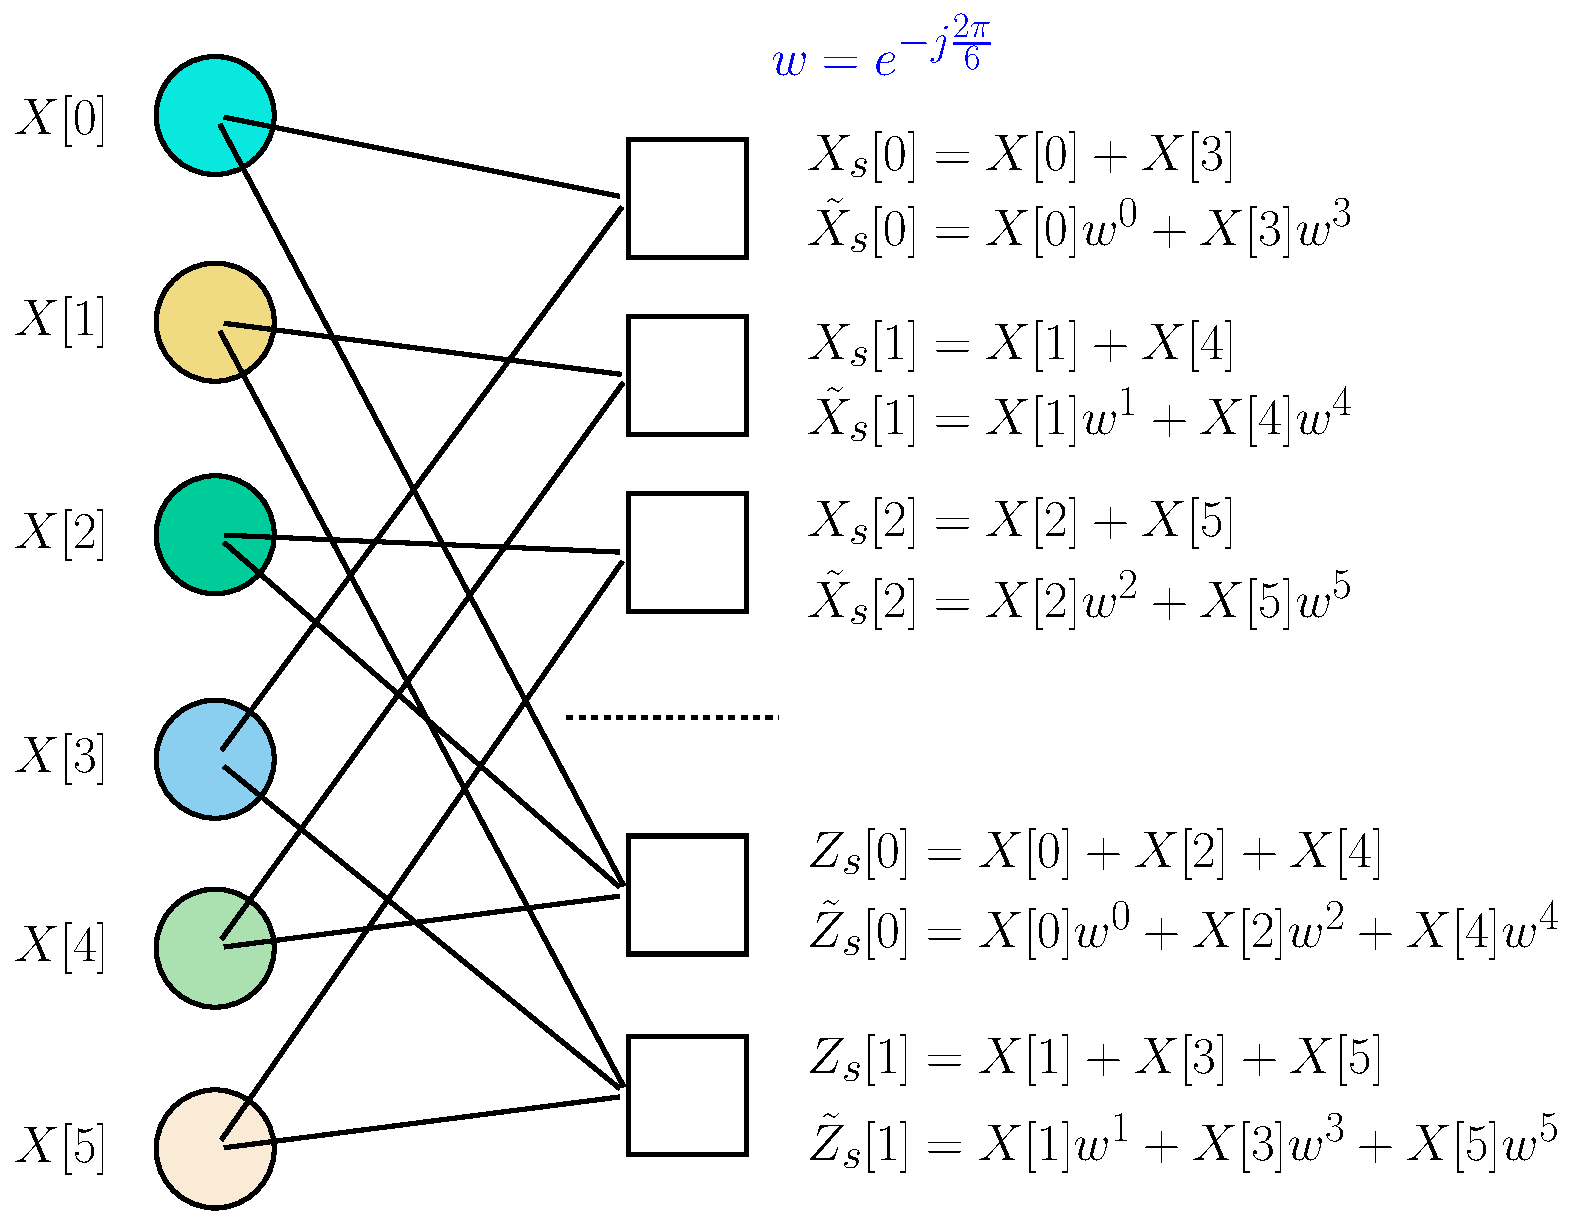
\includegraphics[width=2.75in]{./Figures/Factorgraph_example_tilde}
%			\end{figure}
		\begin{block}{Reed Solomon component codes}
			\begin{itemize}
				\item $(X_s[l_1],\tilde{X}_s[l_1])$ correspond to 2 syndromes of a 1-error correcting RS code
                \item RS is over the complex field, no miscorrection
			\end{itemize}
		\end{block}
	\end{frame}	
	%--------------------------------------------------------------------------------------
	\begin{frame}{Product codes and FFAST ($d=2$)}
	%\begin{itemize}
	%	\item Aliasing equations
	%	\item Mapping (CRT ensures bijective property)
	%	\item Figure: Example 5x4  PC matrix showing how the elements are arranged
	%\end{itemize}
	
	\begin{itemize}
		\item \alert{$X$}: \ $K$-sparse spectrum of length $N = P_1 P_2$  ($P_1$ and $P_2$ are co-prime)
		\item \alert{$X'$}: \  $P_1 \times P_2$ matrix formed by rearranging $X$ according to mapping $\mathcal{M}$	
	\end{itemize}
	
	\begin{columns}
		
		\column{.6\textwidth}
		\begin{block}{}
			\scriptsize{
				\begin{eqnarray}\nonumber
				{\color{blue}X_s[l_1]} & = & \sum_{i=0}^{P_2-1} X[l_1+iP_1], \ \ \ 0 \leq l_1 \leq P_2-1  \label{eqn:Xs_equation} \\ \nonumber
				{\color{blue}Z_s[l_2]} & = & \sum_{i=0}^{P_1-1} X[l_2+iP_2], \ \ \  0 \leq l_2 \leq P_1-1  \label{eqn:Zs} \nonumber
				\end{eqnarray} }	
		\end{block}
		
		\begin{block}{Mapping}
	The mapping from $X(r)$ to $X'(i,j)$ is given by
	\[\color{blue}
	(i,j) = \mathcal{M}(r) \equiv (r \mod P_2, \ r \mod P_1).
	\]
	\alert{Note:} CRT ensures that $\mathcal{M}$ is \textcolor{blue}{bijective}
	    \end{block}
	
	
	\column{.4\textwidth}
	
	\begin{figure}[t]
		\centering
		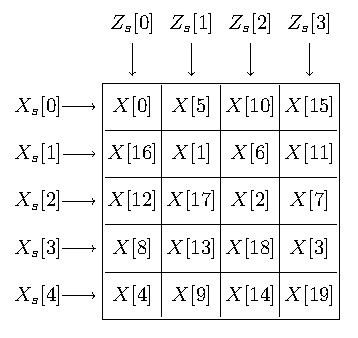
\includegraphics[width=1.8in]{./Figures/ProductCodesMatrix}	
	\end{figure}
	
	\end{columns}
	\end{frame}
	%---------------------------------------------------------------------------------------
	\begin{frame}{Product codes and FFAST ($d \geq 3$)}
	%	\begin{itemize}
	%		\item Mapping equations for less-sparse and very-sparse regimes.
	%		\item Figures: Less-sparse regime and Very-sparse regime 3-D PC structure and highlighting one component code (line and a plane)
	%	\end{itemize}
	\color{blue}$N= P_1 \times P_2 \times \ldots \times P_d$
	
	\[\color{blue} (i_1,i_2,\ldots, i_d) = \mathcal{M}(r) \equiv (r \mod f_1, r \mod f_2, \ldots, r \mod f_d ).
	\]
	
	\begin{columns}
		\column{.45\textwidth}
		\begin{block}{Less-sparse regime}
			\color{red} $f_i= N/P_i,\ i=1,2, \ldots,d$\\ \vspace{0.2in}
			\vspace{-2mm}
			\color{blue} $\underline{d=3}$
			\vspace{-3mm}
			\begin{figure}[t]
				\centering
				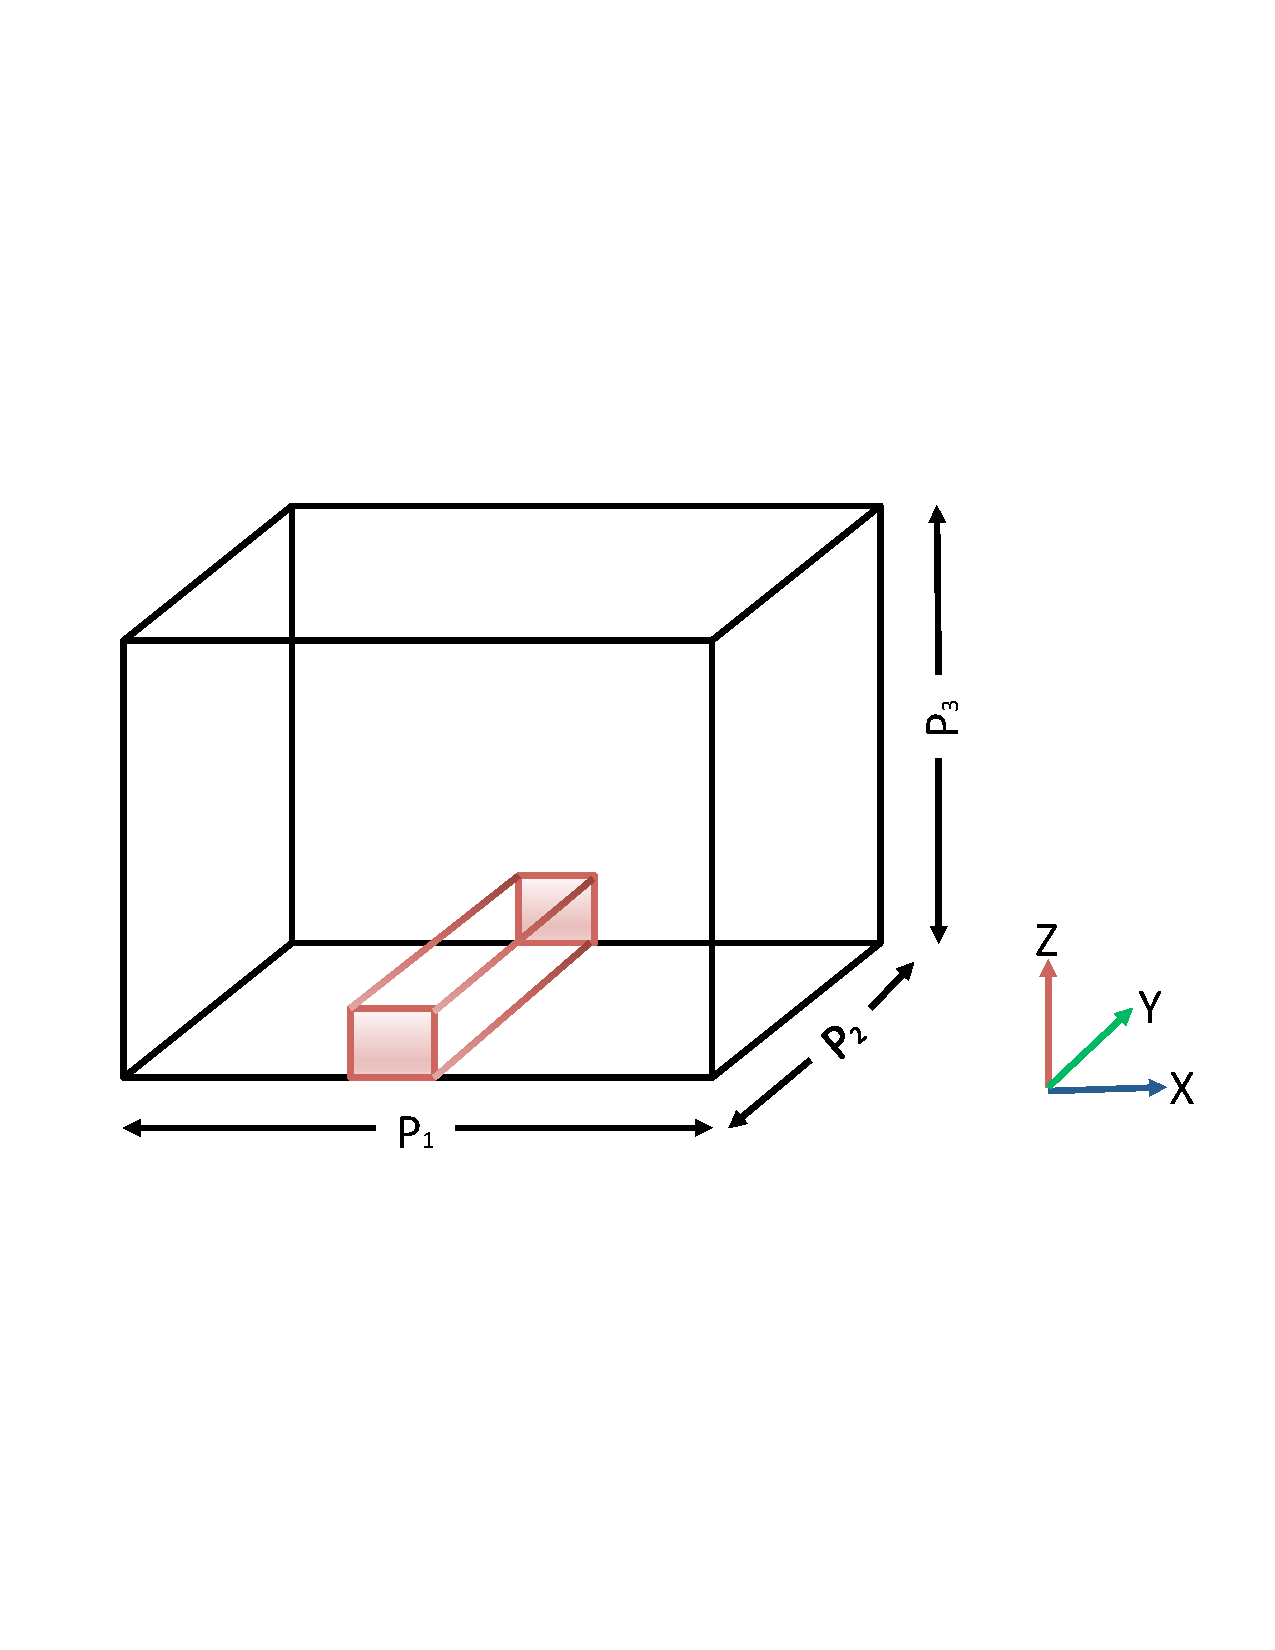
\includegraphics[width=2.2in]{./Figures/less-sparse}
			\end{figure}
			
		\end{block}
		\column{.45\textwidth}
		\begin{block}{Very-sparse regime}
			\color{red} $f_i= P_i,\ i=1,2, \ldots,d$\\ \vspace{0.2in}
			\vspace{-2mm}
			\color{blue} $\underline{d=3}$
			\vspace{-3mm}
			\begin{figure}[t]
				\centering
				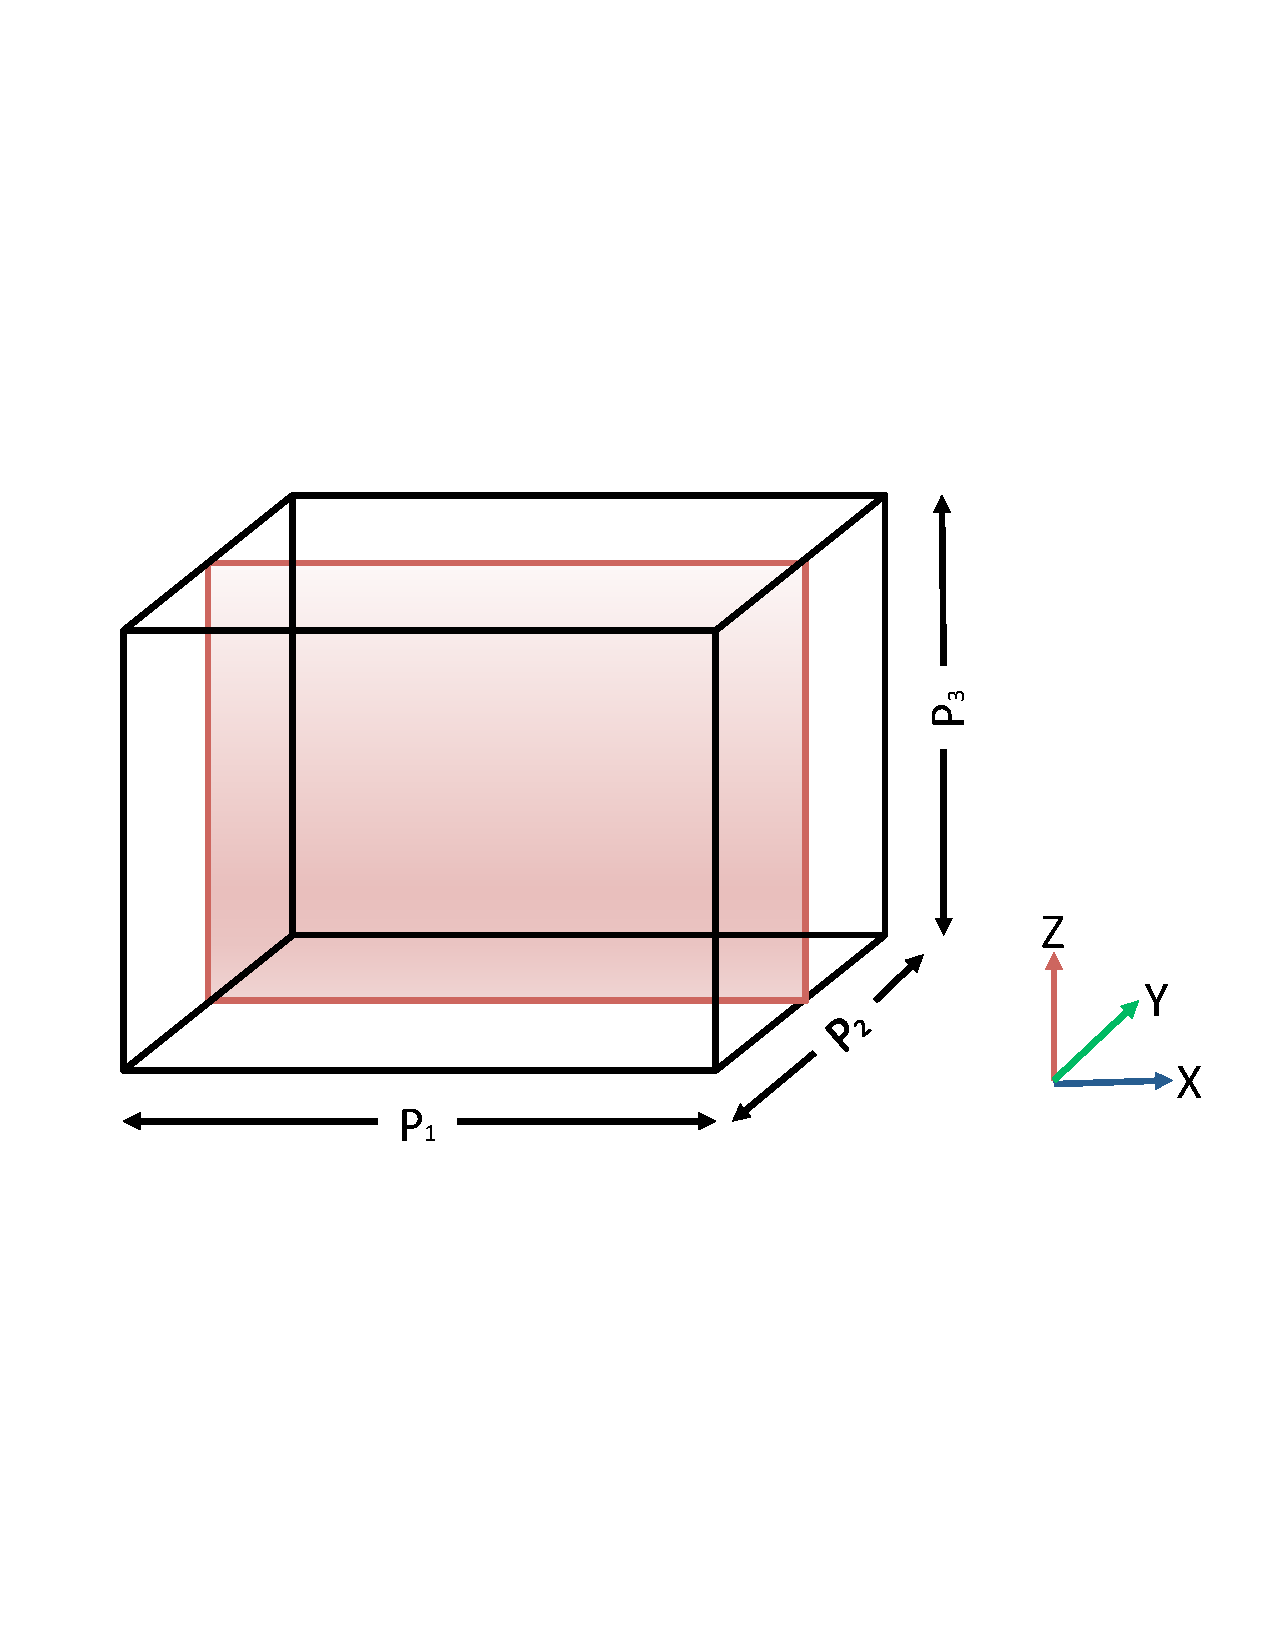
\includegraphics[width=2.2in]{./Figures/very-sparse}
			\end{figure}
			
		\end{block}
	\end{columns}
		
		
	\end{frame}
	%---------------------------------------------------------------------------------------
%	\begin{frame}{Analysis of FFAST using LDPC codes}
%		\begin{itemize}
%			\item Let $n=\prod_{i=0}^{2}f_i$
%			\item Consider $k = O(n^{1/3})$, and $\mathcal{F}={f_0,f_1,f_2}$ be the set of pairwise co-primes.
%			\item Let $f_i = O(k)$ and no. of samples $m = \sum_{i=0}^{2}f_i$			\end{itemize}
%		
%		\begin{block}{Randomized construction: {\color{blue} $\mathcal{C}_{1}^{k}(\mathcal{F},m)$}}
%		\begin{itemize}
%			\item Ensemble of bipartite graphs with $k$ variable nodes and $m$ checknodes
%			\item Partition set of $m$ checknodes into 3 subsets of $f_0$, $f_1$ and $f_2$ nodes
%			\item Each variable node is connected to one checknode from each set, uniformly at random
%		\end{itemize}
%		\end{block}
%		
%		\begin{block}{CRT based construction: {\color{blue} $\mathcal{C}_{2}^{k}(\mathcal{F},n)$}}
%			\begin{itemize}
%				\item Ensemble of bipartite graphs with $k$ variable nodes(selected randomly from $n$ variable nodes) and $m$ checknodes
%				\item Let $\mathcal{I}$ be the set of integers that denote the positions of the $k$ variable nodes.
%				\item Partition set of $m$ checknodes into 3 subsets of $f_0$, $f_1$ and $f_2$ nodes
%				\item Each variable node with an associated integer $v \in \mathcal{I}$ is connected to checknode \alert{$v \mod f_i$} from set $i$.
%			\end{itemize}
%		\end{block}
%		
%	\end{frame}
	%------------------------------------------------------------------------------------
%	\begin{frame}{Analysis of FFAST using LDPC codes}
%		\begin{block}{Lemma}
%			The ensemble of bipartite graphs $\mathcal{C}_{1}^{k}(\mathcal{F},m)$ is identical to the ensemble $\mathcal{C}_{2}^{k}(\mathcal{F},n)$).
%		\end{block}
%		
%		\begin{block}{Main Idea}
%			\begin{itemize}
%				\item Analysis of peeling decoder over $\mathcal{C}_{1}^{k}(\mathcal{F},m)$ is same as analysis of FFAST performance.
%			    \item Density Evolution (DE)  for $\mathcal{C}_{1}^{k}(\mathcal{F},m)$ is well studied.
%			\end{itemize}
%			
%		\end{block}
%	\end{frame}
	%---------------------------------------------------------------------------------------
	\begin{frame}{Connections between FFAST and Product Codes}
	%	Slide-1:
	%	\begin{itemize}
	%		\item Parallel comparison of FFAST and PC and what each parameter in the generalized FFAST correspond to in PC.
	%    \end{itemize}
	%    Side-2:
	%    \begin{itemize}
	%    	\item List the advantages of establishing this connection.
	%    \end{itemize}
	 \only<1>{\begin{columns}
	 	\column{0.50\textwidth}
	 	\begin{figure}[t]
	 		\centering
	 		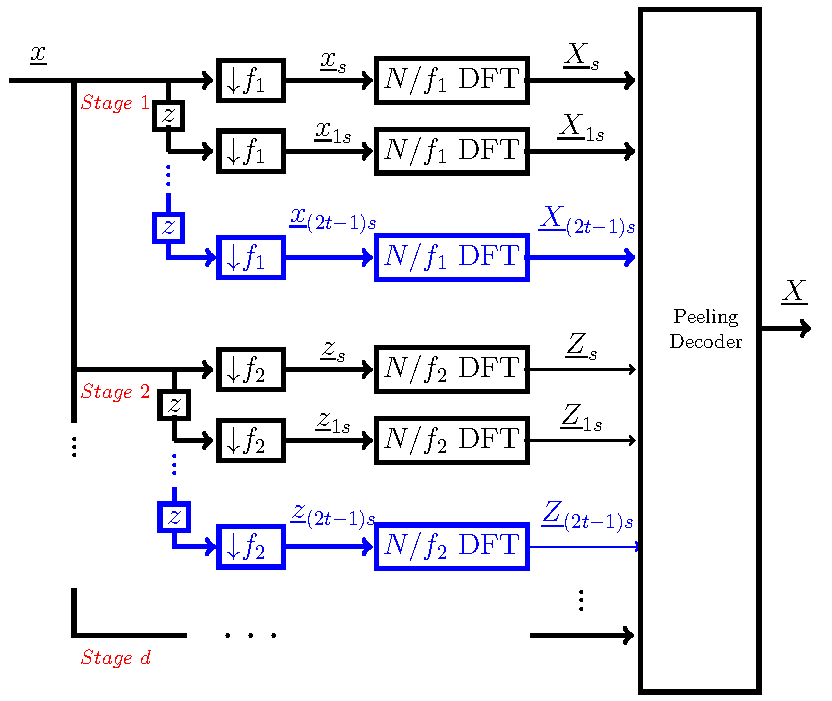
\includegraphics[width=2.2in]{./Figures/FFAST_2stages_generalized}
	 	\end{figure}
	 	\vspace{-6mm}
	 	\hspace{-1.5in}
	 	\column{0.50\textwidth}
	 	
	 	\begin{figure}[t]
	 		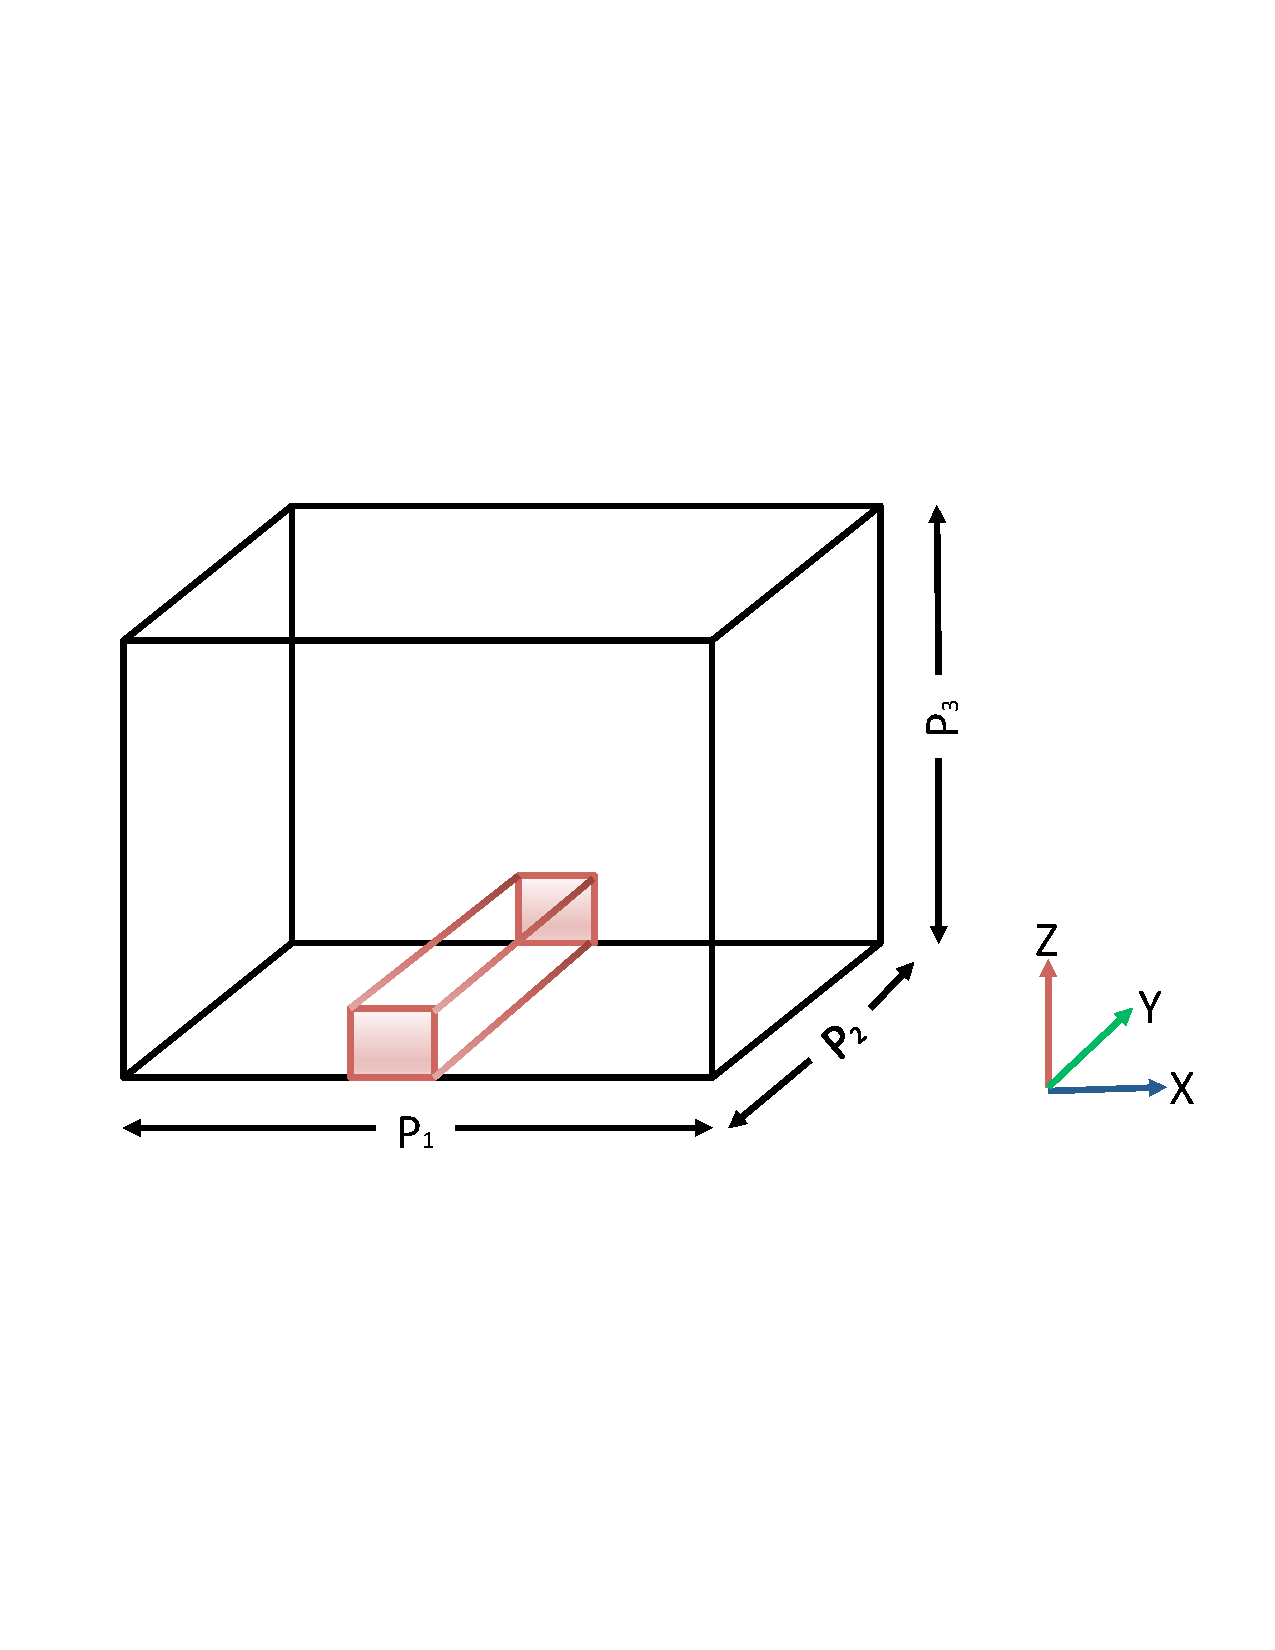
\includegraphics[width=2.4in]{./Figures/less-sparse}
	 	\end{figure}
	 \end{columns}
	
	{\hspace{20 pt} \begin{tabular}{ccc}
	 	FFAST & $\Leftrightarrow$ & Product codes \\
	 	$d$ stages & $\Leftrightarrow$ & $d$-dimensional product code \\
	 	$2t$ branches & $\Leftrightarrow$ & $t$-error correcting RS component codes \\
	 	Non-zero coefficients & $\Leftrightarrow$ & Error locations \\
	 	Recovery of coefficients & $\Leftrightarrow$ & Iterative decoding
	 \end{tabular}}}
%	 \only<2>{
%	 	\begin{block}{Advantages}
%	 		\begin{itemize}
%	 			\item Alternative characterization of thresholds
%	 			\item Insight into improving finite length performance
%	 			\item Bursty non-zero coefficients model can be analyzed using stopping sets
%	 			\item Applications in designing interference tolerant A/D converters
%	 			\item New designs for very high rate product codes
%	 		\end{itemize}   	
%	 	\end{block}}
	 	
	\end{frame}
	%---------------------------------------------------------------------------------------
%	\begin{frame}{Density Evolution(DE) for Product Codes -Justesen et al}
%	%   Slide-1:
%	%   \begin{itemize}
%	%   	\item Introduce the main idea of Justesen's analysis (establish the assumptions in the beginning)
%	%   \end{itemize}
%	%   Slide-2:
%	%   \begin{itemize}
%	%   	\item Tail of the Poisson Distribution. Notion of $\pi_{t}(m)$.
%	%   	\item Effect- of first step of decoding. Equation for the new mean in therms of $\pi_t(M)$.
%	%   \end{itemize}
%	
%	   \begin{columns}
%	   	\column{0.72\textwidth}
%	   	
%	   	\begin{block}{Assumptions}
%	   		
%	   		\begin{itemize}
%	   			\item $P_1=P_2= \ldots =P_d = P$
%	   			\item Errors are \alert{randomly distributed} in rows and columns
%	   			\item If $P \gg t$, \alert{\# errors} in each row/col $\sim$ \alert{Poisson}($M$))
%	   		\end{itemize}
%	   	\end{block}
%	   	\pause
%	   	\begin{block}{Main Idea}
%	   		\begin{itemize}
%	   			%\item Random \alert{bipartite graph} - row and column codes
%	   			\item Removal of \alert{corrected vertices} (degree$\leq t$) from row codes $\Leftrightarrow$ removal of random edges from column codes
%	   			\item \# of errors in row/column changes after each iter
%	   			\begin{itemize}
%	   				\item Track the distribution
%	   				%\item Changes the Poisson parameter ($m(j)$)
%	   				%\item \alert{Threshold} - max. $M$ such that $m(j) \rightarrow 0$ as $j \rightarrow \infty$
%	   			\end{itemize}
%	   			%\item Generalize for $d \geq 2$
%	   		\end{itemize}
%	   	\end{block}
%	   	\column{0.25\textwidth}
%	   	 	
%	   	\begin{figure}[t]
%	   		\centering
%	   		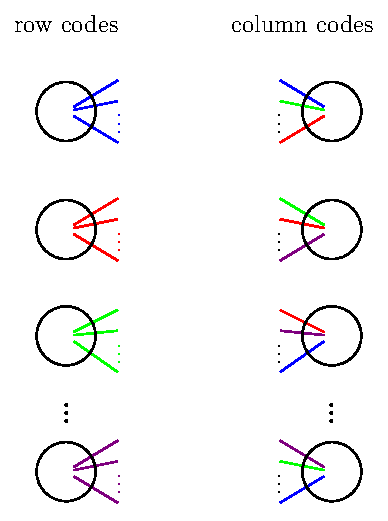
\includegraphics[width=1.3in]{./Figures/Bipartite_graph}
%	   	\end{figure}
%	   		
%	   \end{columns}
%	
%	\end{frame}
	%--------------------------------------------------------------------------------------
%	\begin{frame}{DE continued}
%		\begin{block}{Tail of the Poisson distribution}
%			\begin{equation}\nonumber
%			\pi_t(m) = \sum_{j \geq t} \mathrm{e}^{-m}m^j/j!
%			\label{eqn:defpi}
%			\end{equation}
%		\end{block}
%		
%		\begin{block}{Effect of first step of decoding}
%			If the \# errors is poisson with mean $M$, Mean \# of errors after decoding is
%			\begin{equation}\nonumber
%			\textcolor{blue}{m(1)} = \sum_{j \geq t+1} j\mathrm{e}^{-M}M^j/j! = M\pi_t(M)
%			\label{eqn:defpi}
%			\end{equation}
%		\end{block}
%		
%	\end{frame}
	%----------------------------------------------------------------------------------------
%	\begin{frame}{Evolution of degree distribution($d=2$) - first iteration}
%	
%	%	Slide-1: First iteration
%	%	\begin{itemize}
%	%		\item Figures: Graphs showing how the distribution changes before/after row/column decoding in the first iteration
%	%	\end{itemize}
%	%	Slide-2: jth iteration
%	%	\begin{itemize}
%	%		\item Figures: Degree distribution for jth iteration.
%	%		\item Equations showing the relation between two successive means.
%	%	\end{itemize}
%	
%		\begin{columns}
%			
%			\column{0.5\textwidth}
%			{\vspace{-6mm}
%				\hspace{6mm}
%				\begin{block}{Before row decoding}
%					{\color{blue}Distribution}: Poisson($M$) \\
%					{\color{blue}Mean}: $M$
%				\end{block}}
%				
%				\begin{block}{After row decoding}
%					{\color{blue}Distribution}: Truncated Poisson($M$) \\
%					{\color{blue}Mean}: $M \pi_t(M) = m(1)$
%				\end{block}
%				
%				\begin{block}{Before column decoding}
%					{\color{blue}Distribution}: Poisson($m(1)$) \\
%					{\color{blue}Mean}: $m(1)$
%				\end{block}
%				
%				\begin{block}{After column decoding}
%					{\color{blue}Distribution}: Truncated Poisson($m(1)$) \\
%					%{\color{blue}Mean}: $m(2) = M \pi_t(m(1))$
%				\end{block}
%				
%				
%				\column{0.5\textwidth}
%				\begin{center}
%					\vspace{-3mm}
%					% This file was created by matlab2tikz.
%
%The latest updates can be retrieved from
%  http://www.mathworks.com/matlabcentral/fileexchange/22022-matlab2tikz-matlab2tikz
%where you can also make suggestions and rate matlab2tikz.
%
\definecolor{mycolor1}{rgb}{0.00000,0.44700,0.74100}%
%
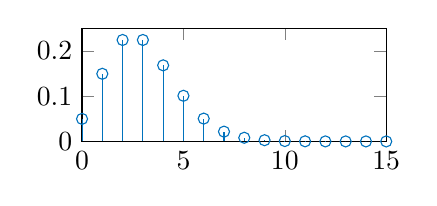
\begin{tikzpicture}

\begin{axis}[%
width=1.521in,
height=0.566in,
at={(0.758in,0.481in)},
scale only axis,
xmin=0,
xmax=15,
ymin=0,
ymax=0.25,
axis background/.style={fill=white}
]
\addplot[ycomb,color=mycolor1,solid,mark=o,mark options={solid},forget plot] plot table[row sep=crcr] {%
0	0.0497870683678639\\
1	0.149361205103592\\
2	0.224041807655388\\
3	0.224041807655388\\
4	0.168031355741541\\
5	0.100818813444924\\
6	0.0504094067224623\\
7	0.0216040314524838\\
8	0.00810151179468143\\
9	0.00270050393156048\\
10	0.000810151179468142\\
11	0.00022095032167313\\
12	5.52375804182826e-05\\
13	1.27471339426806e-05\\
14	2.73152870200298e-06\\
15	5.46305740400597e-07\\
};
\end{axis}
\end{tikzpicture}%
%					% This file was created by matlab2tikz.
%
%The latest updates can be retrieved from
%  http://www.mathworks.com/matlabcentral/fileexchange/22022-matlab2tikz-matlab2tikz
%where you can also make suggestions and rate matlab2tikz.
%
\definecolor{mycolor1}{rgb}{0.00000,0.44700,0.74100}%
%
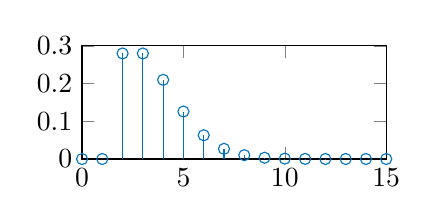
\begin{tikzpicture}

\begin{axis}[%
width=1.521in,
height=0.566in,
at={(0.758in,0.481in)},
scale only axis,
xmin=0,
xmax=15,
ymin=0,
ymax=0.3,
axis background/.style={fill=white}
]
\addplot[ycomb,color=mycolor1,solid,mark=o,mark options={solid},forget plot] plot table[row sep=crcr] {%
0	0\\
1	0\\
2	0.279754460090289\\
3	0.279754460090289\\
4	0.209815845067717\\
5	0.12588950704063\\
6	0.0629447535203151\\
7	0.0269763229372779\\
8	0.0101161211014792\\
9	0.00337204036715975\\
10	0.00101161211014792\\
11	0.000275894211858524\\
12	6.89735529646311e-05\\
13	1.59169737610687e-05\\
14	3.41078009165758e-06\\
15	6.82156018331516e-07\\
};
\end{axis}
\end{tikzpicture}%
%					% This file was created by matlab2tikz.
%
%The latest updates can be retrieved from
%  http://www.mathworks.com/matlabcentral/fileexchange/22022-matlab2tikz-matlab2tikz
%where you can also make suggestions and rate matlab2tikz.
%
\definecolor{mycolor1}{rgb}{0.00000,0.44700,0.74100}%
%
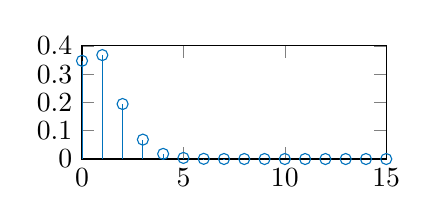
\begin{tikzpicture}

\begin{axis}[%
width=1.521in,
height=0.566in,
at={(0.758in,0.481in)},
scale only axis,
xmin=0,
xmax=15,
ymin=0,
ymax=0.4,
axis background/.style={fill=white}
]
\addplot[ycomb,color=mycolor1,solid,mark=o,mark options={solid},forget plot] plot table[row sep=crcr] {%
0	0.347043782149382\\
1	0.367277938616125\\
2	0.194345917046349\\
3	0.0685590420793257\\
4	0.0181390828359174\\
5	0.00383933399474955\\
6	0.000677197300830985\\
7	0.000102382976886822\\
8	1.35440435164562e-05\\
9	1.59263554985051e-06\\
10	1.68549310433711e-07\\
11	1.62160423332975e-08\\
12	1.43012565633619e-09\\
13	1.16423706136106e-10\\
14	8.80083662455855e-12\\
15	6.20930902636336e-13\\
};
\end{axis}
\end{tikzpicture}%
%					% This file was created by matlab2tikz.
%
%The latest updates can be retrieved from
%  http://www.mathworks.com/matlabcentral/fileexchange/22022-matlab2tikz-matlab2tikz
%where you can also make suggestions and rate matlab2tikz.
%
\definecolor{mycolor1}{rgb}{0.00000,0.44700,0.74100}%
%
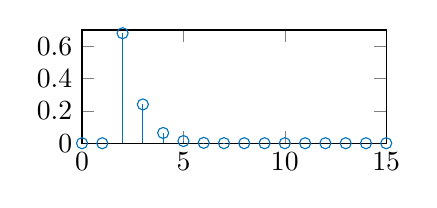
\begin{tikzpicture}

\begin{axis}[%
width=1.521in,
height=0.566in,
at={(0.758in,0.481in)},
scale only axis,
xmin=0,
xmax=15,
ymin=0,
ymax=0.7,
axis background/.style={fill=white}
]
\addplot[ycomb,color=mycolor1,solid,mark=o,mark options={solid},forget plot] plot table[row sep=crcr] {%
0	0\\
1	0\\
2	0.680296442442702\\
3	0.23998689106868\\
4	0.0634947917094919\\
5	0.0134393626461139\\
6	0.00237048928832011\\
7	0.000358385583815417\\
8	4.74101270588406e-05\\
9	5.57492699171389e-06\\
10	5.89996939513159e-07\\
11	5.67633016299058e-08\\
12	5.0060706756166e-09\\
13	4.07534330044602e-10\\
14	3.08068105427641e-11\\
15	2.17353207356291e-12\\
};
\end{axis}
\end{tikzpicture}%
%				\end{center}
%				
%			\end{columns}
%		\end{frame}
	%------------------------------------------------------------------------------------------
%		\begin{frame}{Evolution of degree distribution - $j$th iteration}
%			\begin{columns}
%				
%				\column{0.55\textwidth}
%				{\vspace{-6mm}
%					\hspace{6mm}
%					\begin{block}{Before row decoding}
%						{\color{blue}Distribution}: Poisson($m(j)$) \\
%					\end{block}}
%					\vspace{6mm}
%					\begin{block}{After row decoding}
%						{\color{blue}Distribution}: Truncated Poisson($m(j)$) \\
%						{\color{blue}Mean}: $m(j) \pi_t(m(j))$ \\
%						{\color{blue}Reduction by a factor}: $\frac{m(j) \pi_t(m(j))}{m(j-1) \pi_t(m(j-1))}$ \\
%					\end{block}
%					\column{0.45\textwidth}
%					\begin{center}
%						\vspace{-3mm}
%						% This file was created by matlab2tikz.
%
%The latest updates can be retrieved from
%  http://www.mathworks.com/matlabcentral/fileexchange/22022-matlab2tikz-matlab2tikz
%where you can also make suggestions and rate matlab2tikz.
%
\definecolor{mycolor1}{rgb}{0.00000,0.44700,0.74100}%
%
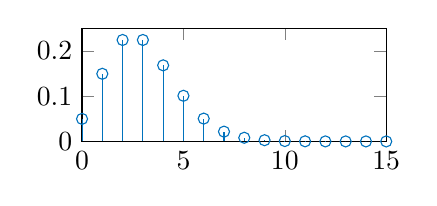
\begin{tikzpicture}

\begin{axis}[%
width=1.521in,
height=0.566in,
at={(0.758in,0.481in)},
scale only axis,
xmin=0,
xmax=15,
ymin=0,
ymax=0.25,
axis background/.style={fill=white}
]
\addplot[ycomb,color=mycolor1,solid,mark=o,mark options={solid},forget plot] plot table[row sep=crcr] {%
0	0.0497870683678639\\
1	0.149361205103592\\
2	0.224041807655388\\
3	0.224041807655388\\
4	0.168031355741541\\
5	0.100818813444924\\
6	0.0504094067224623\\
7	0.0216040314524838\\
8	0.00810151179468143\\
9	0.00270050393156048\\
10	0.000810151179468142\\
11	0.00022095032167313\\
12	5.52375804182826e-05\\
13	1.27471339426806e-05\\
14	2.73152870200298e-06\\
15	5.46305740400597e-07\\
};
\end{axis}
\end{tikzpicture}%
%						% This file was created by matlab2tikz.
%
%The latest updates can be retrieved from
%  http://www.mathworks.com/matlabcentral/fileexchange/22022-matlab2tikz-matlab2tikz
%where you can also make suggestions and rate matlab2tikz.
%
\definecolor{mycolor1}{rgb}{0.00000,0.44700,0.74100}%
%
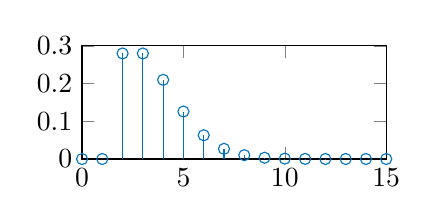
\begin{tikzpicture}

\begin{axis}[%
width=1.521in,
height=0.566in,
at={(0.758in,0.481in)},
scale only axis,
xmin=0,
xmax=15,
ymin=0,
ymax=0.3,
axis background/.style={fill=white}
]
\addplot[ycomb,color=mycolor1,solid,mark=o,mark options={solid},forget plot] plot table[row sep=crcr] {%
0	0\\
1	0\\
2	0.279754460090289\\
3	0.279754460090289\\
4	0.209815845067717\\
5	0.12588950704063\\
6	0.0629447535203151\\
7	0.0269763229372779\\
8	0.0101161211014792\\
9	0.00337204036715975\\
10	0.00101161211014792\\
11	0.000275894211858524\\
12	6.89735529646311e-05\\
13	1.59169737610687e-05\\
14	3.41078009165758e-06\\
15	6.82156018331516e-07\\
};
\end{axis}
\end{tikzpicture}%
%					\end{center}
%			\end{columns}
%				
%				
%				\begin{block}{d-stages}
%					
%					\begin{center}
%						\begin{itemize}
%							\item  $m(j)= M \ \prod \limits_{i=1}^{d-1}{\pi_t(m(j-i))}$
%							\item $\frac{m(j)}{m(j-d)}=\frac{M\prod\limits_{i=1}^{d-1} \pi_t(m(j-i))}{m(j-d)} \leq M \frac{\pi_t^{d-1}(m(j-d))}{m(j-d)}$
%						\end{itemize}
%					\end{center}
%					
%				\end{block}
%			\end{frame}

	%----------------------------------------------------------------------------------------
	\begin{frame}{Thresholds}
	%	\begin{itemize}
	%		
	%	\item Theorem for the Threshold value for Less-sparse case.
	%	\item Table showing threshold values for different $d$ and $t$.
	%	\item Highlight some useful points in the table {\bf(if needed)}
	%	\end{itemize}
		
		\begin{theorem}\label{thm:thresh}
			Less sparse case: In the limit of large $P$, the FFAST algorithm with $d$ branches and $2t$ stages can recover the FFT coefficients w.h.p if $K < \frac{2dt}{c_{d,t}}$. \\
			\vspace{2mm}
			\centering
			\color{blue} $c_{d,t} = \min_m \{ m / \pi^{d-1}(m)\} $
		\end{theorem}
		
		\begin{block}{}
			
			\begin{center}
				\alert{Threshold} = $ \frac{\# \ of \ measurements}{recoverable \ sparsity}={\color{blue} \frac{2dt}{c_{d,t}}}$
			\end{center}
			
			\vspace{-6mm}
			\color{black}
			\begin{table}[ht]
				\centering
				\begin{tabular}{c|ccccccc}
					\hline
					& $d=2$ & $d=3$ & $d=4$ & $d=5$ & $d=6$ & $d=7$ & $d=8$ \\
					\hline
					\rowcolor{lightgray}
					$t=1$& 4.0  & 2.4436 & 2.5897 & 2.8499 & 3.1393 & 3.4378 & 3.7383 \\
					$t=2$& 2.3874 & 2.5759 & 2.9993 & 3.4549 & 3.9153 & 4.3736 & 4.8278 \\
					\rowcolor{lightgray}
					$t=3$& 2.3304 & 2.7593 & 3.3133 & 3.8817 & 4.4483 & 5.0094 & 5.5641 \\
					$t=4$& 2.3532 & 2.9125 & 3.5556& 4.2043 & 4.8468 & 5.4802 & 6.1033 \\
					%\rowcolor{lightgray}
					%$t=5$& 2.3908 & 3.0394 & 3.7471 & 4.4500 & 5.1362 & 5.8018 & 6.4451 \\
					
					\hline
				\end{tabular}
			\end{table}
			\vspace{-3mm}
			
			Notice that $L,K = O \left( N^{\frac{1-d}{d}}\right)$
		\end{block}
		
		
	\end{frame}
	%-----------------------------------------------------------------------------------------
%	\begin{frame}\frametitle{Bursty signals}
%	%	Slide-1: Introduce bursty signals setup and notations. \\
%	%	Slide-2: One burst case
%	%	\begin{itemize}
%	%		\item Theorem:  \# of errors recoverable for $d=2$ and $b=1$.
%	%		\item Figure: Example to explain the theorem.
%	%	\end{itemize}
%	%	Slide-3: Two burst case
%	%	\begin{itemize}
%	%		\item Theorem and Conjecture:  \# of errors recoverable for $d=2$ and $b=2$.
%	%		\item Proof {\bf(if required)}
%	%	\end{itemize}
%	%	
%		
%		
%		
%		\begin{block}{Bursty Signals}
%			Signals that have non-zero Fourier coefficients occurring in bursts. Let $b$ be the number of bursts.
%		\end{block}
%		
%		\begin{figure}[t]
%			\centering
%			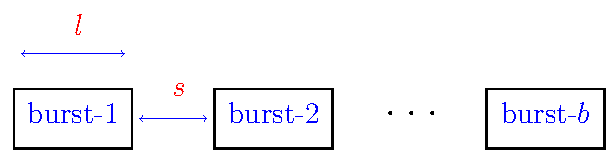
\includegraphics[width=3.0in]{./Figures/burst_spacing}
%		\end{figure}
%		
%	\end{frame}
%	%----------------------------------------------------------------------------------------
%	\begin{frame}\frametitle{One burst case $b=1$}
%		
%		\begin{theorem}
%			\color{blue} For any finite $N$ and $d=2$, $b=1$, any burst of length $K \leq P_1+P_2-1$ is guaranteed to be recoverable
%			
%			\begin{columns}
%				\column{.40\textwidth}
%				
%				\begin{figure}[t]
%					\centering
%					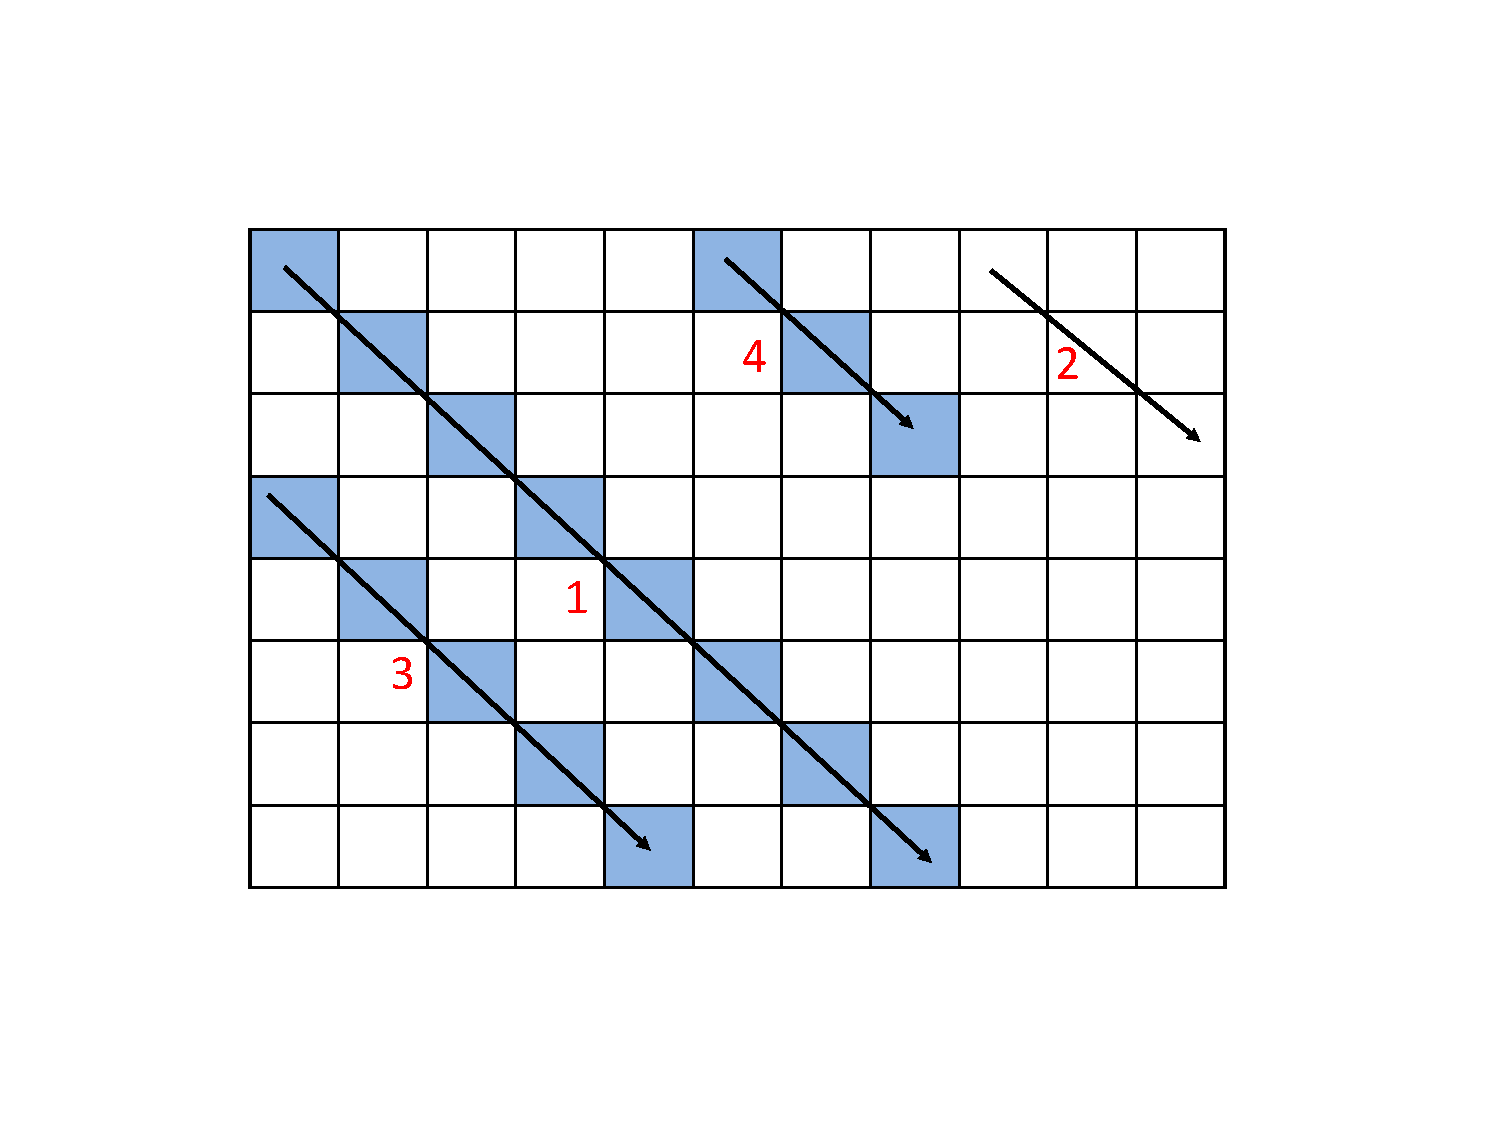
\includegraphics[width=1.9in]{./Figures/1burstmatrix}
%				\end{figure}
%				
%				\column{.55\textwidth}
%				\begin{proof}
%					\begin{itemize}
%						
%						
%						\item WLOG, assume the burst starts at $(0,0)$ (due to cyclic shift property of DFT)
%						\item Paths \alert{1} and \alert{2} cover all columns once.
%						\item Paths \alert{3} and \alert{4} cover all rows once
%						\item So minimum burst length leading to stopping set (\alert{1 + 2 + 3 + 4})= $P_1 + P_2$
%					\end{itemize}
%					
%				\end{proof}
%			\end{columns}
%		\end{theorem}
%	\end{frame}
%	
%	%-------------------------------------------------------------------------------------
%	
%	\begin{frame} \frametitle{Bursty signals (b=2) cont.}
%		
%		\begin{theorem}
%			\color{blue} For any finite $N = P_1 P_2 \ (P_1 > P_2)$, $d=2$ and $b=2$, all bursts of length $l \leq P_2/2$ are recoverable.
%		\end{theorem}
%		
%		\begin{block}{Conjecture}
%			\color{blue} As $N \rightarrow \infty$, for $d=2$, $b=2$, the fraction of bursts of length $K \leq P_1+P_2-1$ that are not recoverable vanishes as $N \rightarrow \infty$.
%		\end{block}
%		
%		\pause
%		\begin{block}{}
%			This means that a threshold exists even for $d=2$ and $t=1$ in the bursty case
%		\end{block}
%	\end{frame}
%	%------------------------------------------------------------------------------------------
%	\begin{frame}{Noise Robust FFAST}
%		\begin{figure}[t]
%			\centering
%			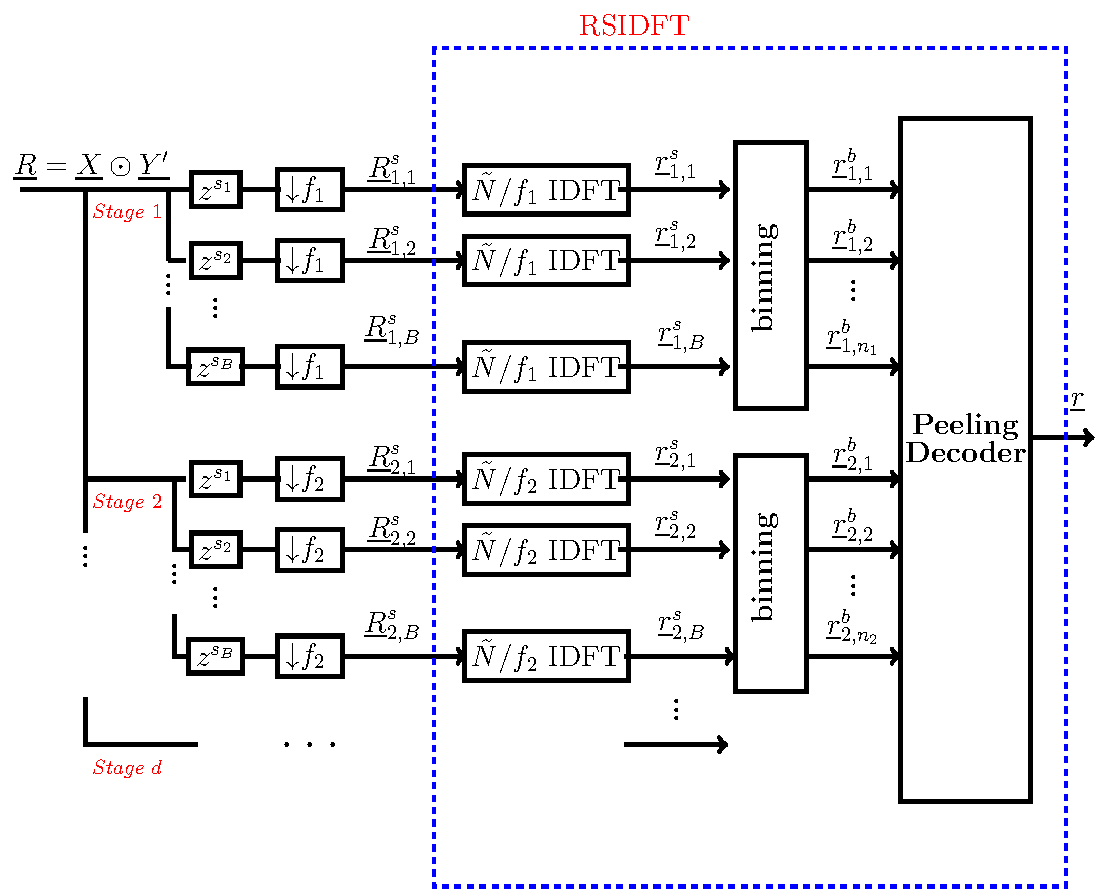
\includegraphics[width=2.5in]{./Figures/FFAST_Robust}
%		\end{figure}
%		\vspace{-0.4cm}
%		\begin{block}{}
%			\begin{itemize}
%				\item $l = O(\log(n))$ branches per stage
%				\item Shifts $s_1, s_2, \ldots s_l$ are chosen such that measurement matrix satisfy
%				    \begin{itemize}
%				    	\item {\color{blue}Mutual incoherence} - level of correlation between two columns
%				    	\item {\color{blue}Restricted isometry} - measures norm preserving capability.
%				    \end{itemize}
%				 	    \item Sample complexity: {\color{blue} $O(k \log n)$}
%				 	    \item Computational complexity: {\color{blue} $ O(n \log n)$}
%				
%				
%			\end{itemize}
%		\end{block}
%	\end{frame}
	%------------------------------------------------------------------------------------------
	\begin{frame}{Interference-tolerant A/D Converter}
		
	%	\begin{itemize}
	%		\item Figure that shows the inherent sparsity in sensed spectrum
	%		\item Simple block diagram of the proposed setup.
	%		\item New slide: Include about the sampling vs latency trade-off. Provide examples to explain the situation {\bf (if needed)}
	%	\end{itemize}
		
		\begin{figure}[t]
			\centering
			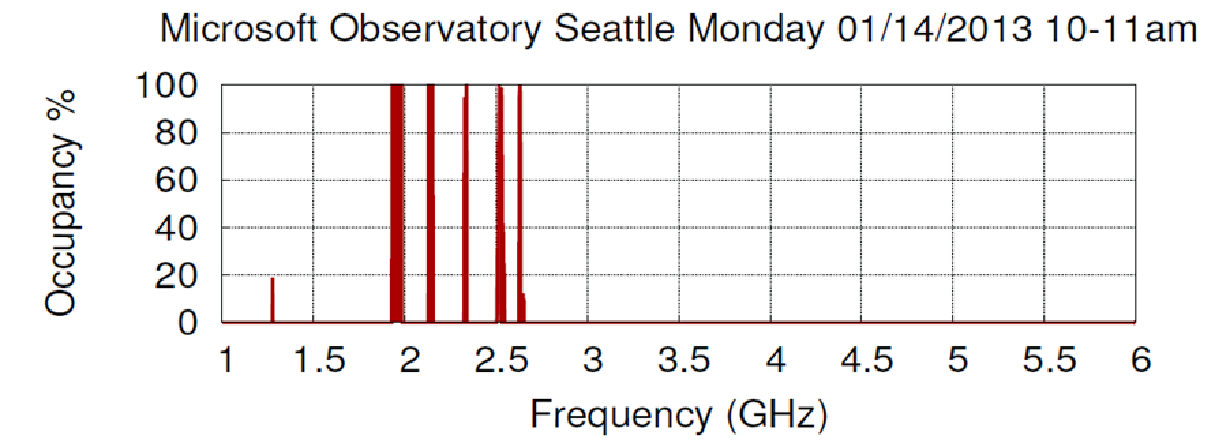
\includegraphics[width=3.5 in]{./Figures/spectrumsensing}
		\end{figure}
		\begin{figure}[t]
			\centering
			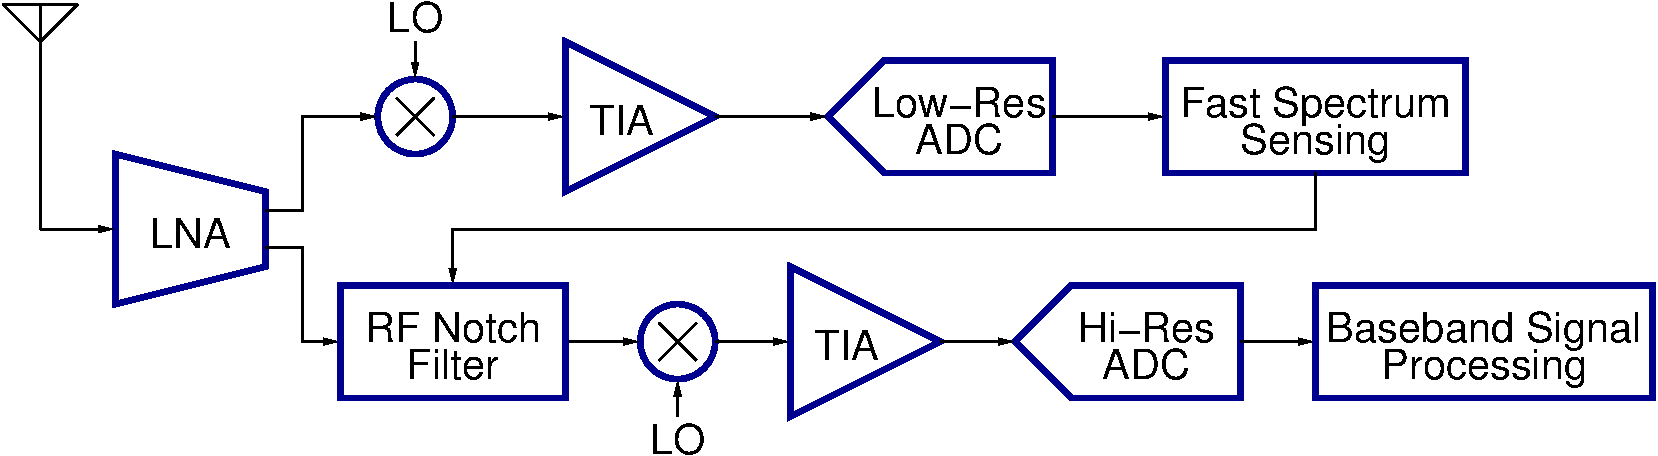
\includegraphics[width=3.5 in]{./Figures/systemdiagram}
		\end{figure}
	\end{frame}
	%------------------------------------------------------------------------------------------
%	\begin{frame}{Simulation results}
%		
%	%	\begin{itemize}
%	%		\item Slide-1: Bursty case better than random
%	%		\item Slide-2: Finite length effects
%	%	\end{itemize}
%		
%		\begin{figure}[t]
%			\centering
%			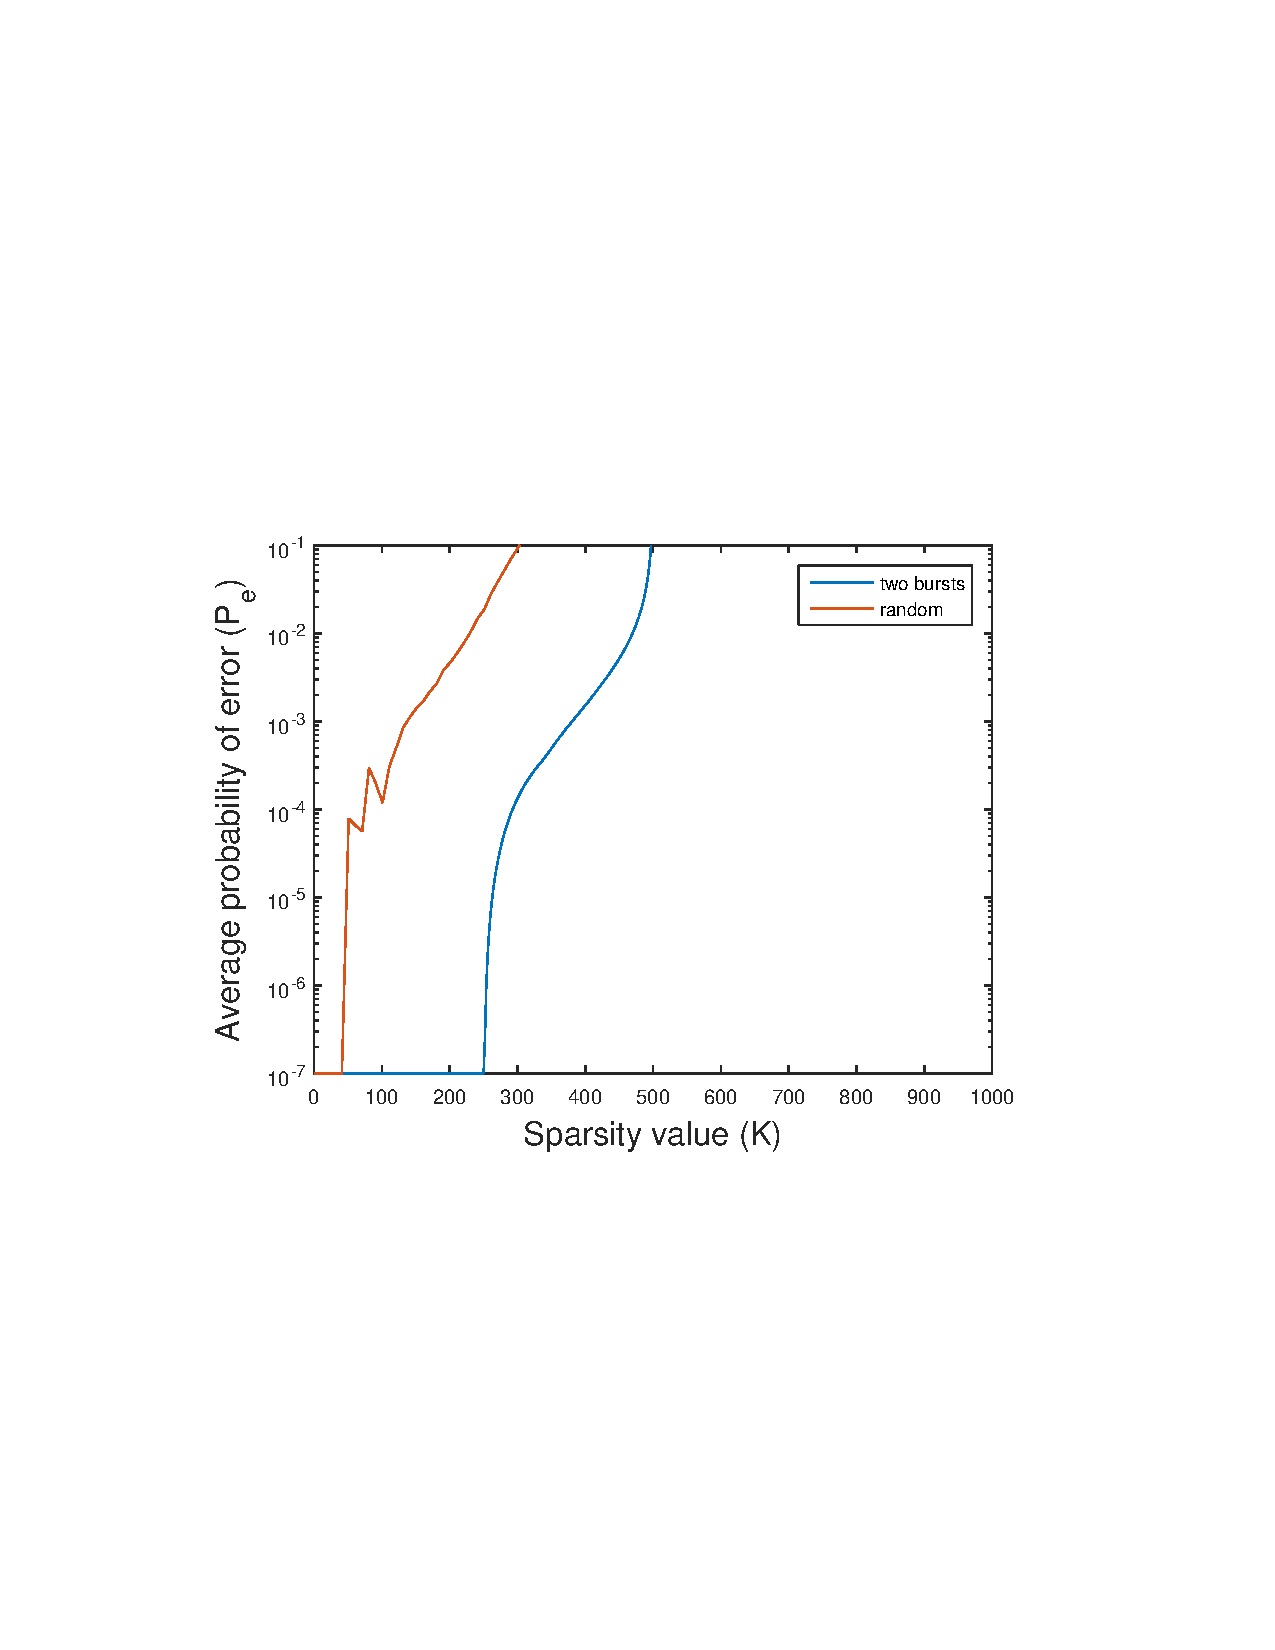
\includegraphics[width=3.5 in]{./Figures/Average_Perror_K_250_251_semilog.pdf}
%			\vspace{-4mm}
%			\caption{Plot of the average probability of error , $P_e$, as a function of the sparsity value, $K$, for bursty and random selection of non-zero coefficients; $N=250\times251$, 1002 samples}
%			\label{fig:probofsuccess250_251}
%		\end{figure}
%		
%	\end{frame}
%	%------------------------------------------------------------------------------------------
%	\begin{frame}{Simulation results for $N \approx 10000$}
%		\begin{figure}[t]
%			\centering
%			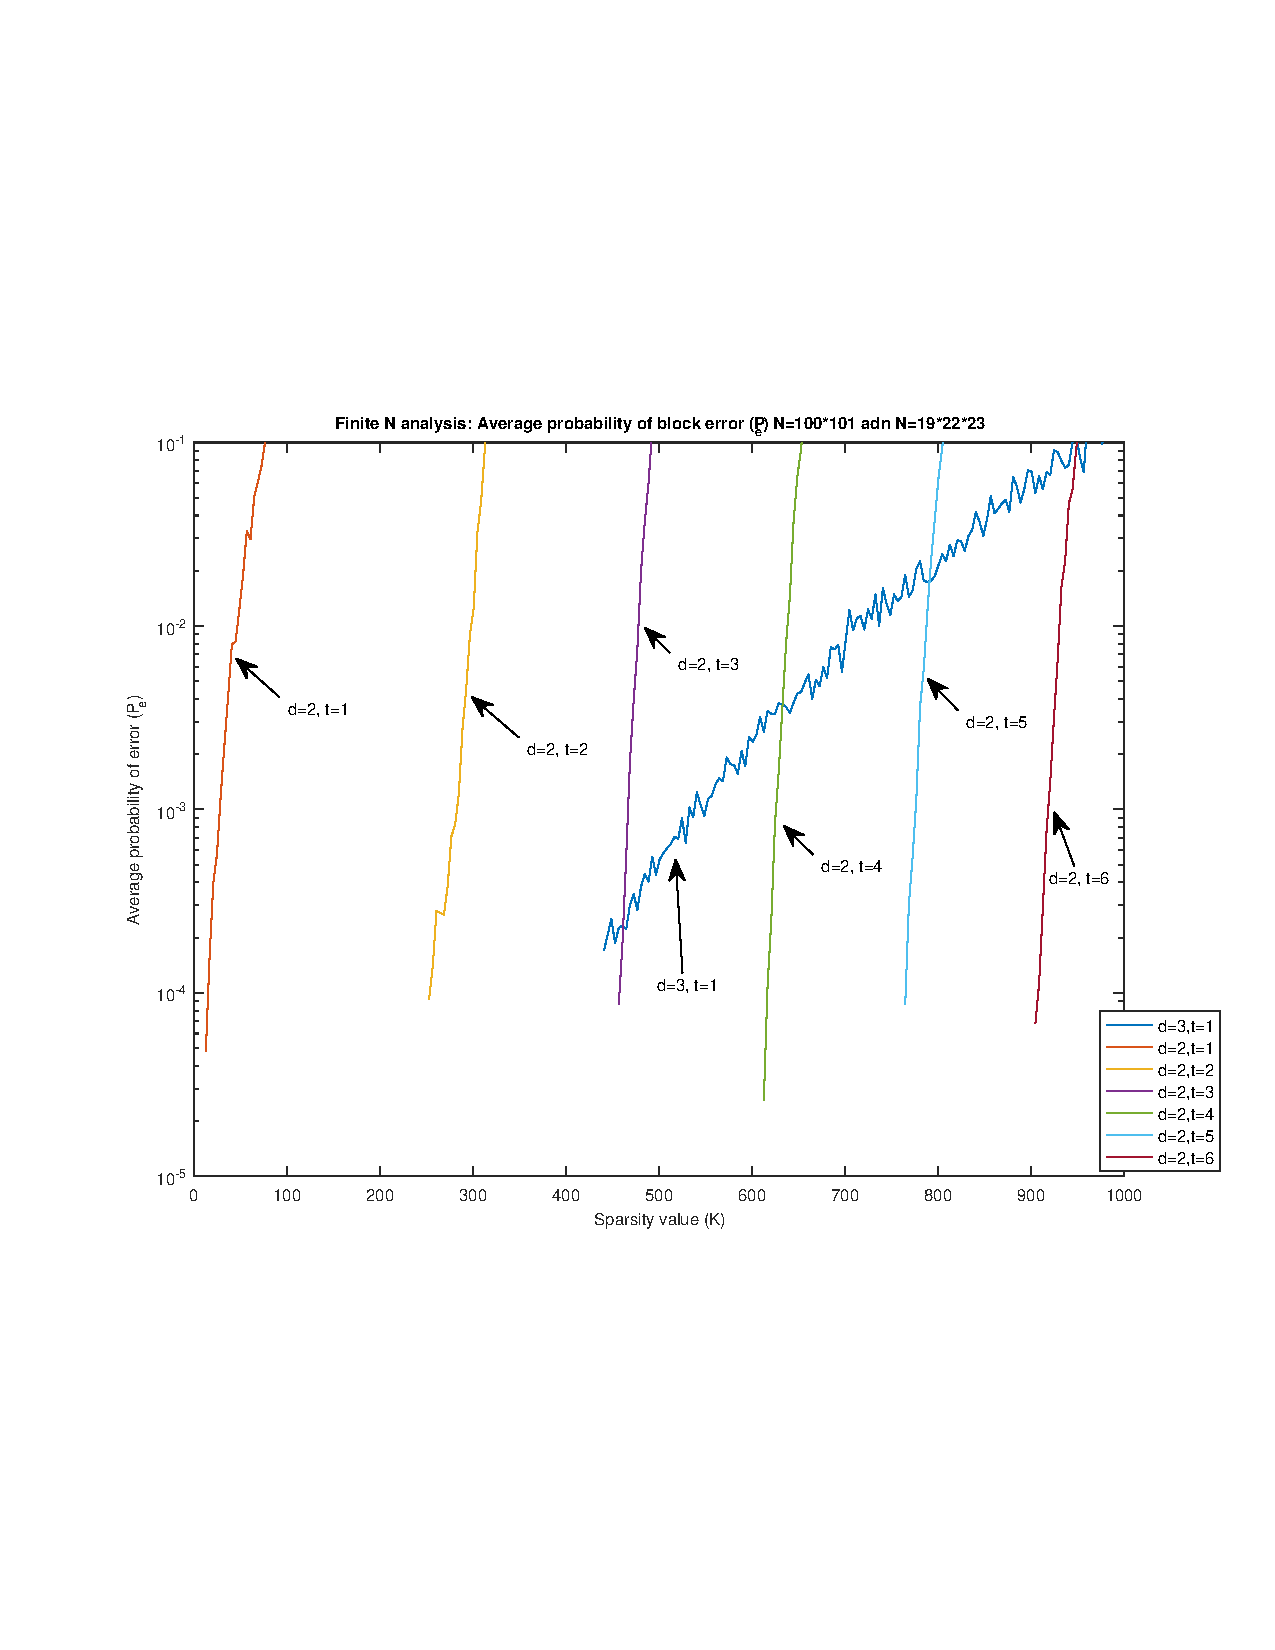
\includegraphics[width=3.9 in]{./Figures/Finite_N_analysis_block}
%		\end{figure}
%		
%	\end{frame}
\begin{frame}{Open problems}
\begin{itemize}
  \item If we use MAP decoding, is the subsampling procedure optimal?
  \item What happens when $N=2^i$ ?
  \item Bursty case? Can we have threshold theorems?
  \item Using this idea in actual applications
\end{itemize}
\end{frame}
 